Fix $ \latentmdp_{\decoderparameter} = \tuple{\latentstates, \latentactions, \latentprobtransitions_{\decoderparameter}, \latentrewards_{\decoderparameter}, \latentlabels, \atomicprops, \zinit}$ and $\tuple{\latentmdp_{\decoderparameter}, \embed_{\encoderparameter}, \embeda_{\decoderparameter}}$ as a latent space model of $\mdp$ parameterized by $\encoderparameter$ and $\decoderparameter$.
Our method relies on learning a \emph{behavioral model}
% $\decoder$
$\stationary{\decoderparameter}$
of $\mdp$ from which we can retrieve the latent space model 
% the parameters of $\latentmdp_{\decoderparameter}$
and distill $\pi$.
This can be achieved via the minimization of a suitable discrepancy between $\stationarydecoder$ and
%a distribution describing the dynamics of $\mdp_\policy$.
% a trace distribution of 
$\mdp_\policy$.
%$\decoder$.
% $\stationary{\decoderparameter}$.
% \begin{equation}
%     \min_{\decoderparameter}D\fun{{\mdp_\policy}, {\decoder}}. \label{eq:discrepancy}
% \end{equation}
%As mentioned in \citep{DBLP:journals/corr/abs-2112-09655},
VAE-MDPs optimize a lower bound on the likelihood of the dynamics of $\mdp_\policy$ using the \emph{Kullback-Leibler divergence},
%one can exploit the VAE framework \cite{DBLP:journals/jmlr/HoffmanBWP13, DBLP:journals/corr/KingmaW13} to
yielding (i) $\latentmdp_{\decoderparameter}$, (ii) a distillation  $\latentpolicy_{\decoderparameter}$ of $\policy$, and (iii) $\embed_{\encoderparameter}$ and $\embeda_{\decoderparameter}$.
%
Local losses are not directly minimized, but rather variational proxies that do not offer theoretical guarantees during the learning process.
%(the log-likelihood of the rewards and the replacement of the Wasserstein term in $\localtransitionloss{\latentpolicy_{\decoderparameter}}$ by $\dklsymbol$) when the latent policy is executed.
To control the local losses minimization and exploit their theoretical guarantees, 
%and avoid this way undesired learning behavior,
we present a novel autoencoder that incorporates them in its objective, derived from the OT. % instead of $\dklsymbol$.
% In the following, we describe how to achieve this goal by considering the minimization of the Wasserstein distance between the .
%
% \subsection{State space abstraction}
Proofs of the claims made in this Section are provided in Appendix~\ref{appendix:wae-mdp}.
\subsection{The Objective Function}
%\smallparagraph{Raw transition distance.}~
Assume that $\states$, $\actions$, and $\images{\rewards}$ are respectively equipped with metrics $\distance_{\states}$, $\distance_{\actions}$, and $\distance_{\rewards}$,
%let us define the \emph{raw transition distance metric} $\transitiondistance$ over 
we define the  \emph{raw transition distance metric} $\transitiondistance$ as the component-wise sum of distances between states, actions, and rewards occurring of along transitions:
$
%\begin{equation}
    \tracedistance\fun{\tuple{\state_1, \action_1, \reward_1, \state'_1}, \tuple{\state_2, \action_2, \reward_2, \state'_2}} = \distance_\states\fun{\state_1, \state_2} + \distance_{\actions}\fun{\action_1, \action_2} + \distance_{\rewards}\fun{\reward_1, \reward_2} + \distance_{\states}\fun{\state_1', \state'_2}.\notag
%\end{equation}
$
%
%possible transitions of $\mdp_\policy$, i.e., tuples of the form $\tuple{\state, \action, \reward, \state', \labeling'}$ such that $\exists \defaulttrace \in \traces{\mdp_\policy}$, $\exists t < T$ with $\tuple{\state, \action, \reward, \state', \labeling'} = \tuple{\state_t, \action_t, \reward_t, \state_{t + 1}, \labeling_{t + 1}}$, as
% \begin{align*}
%     \transitiondistance\fun{\tuple{\state_1, \action_1, \reward_1, \state_1', \labeling_1'}, \tuple{\state_2, \action_2, \reward_2, \state_2', \labeling_2'}} = \distance_{\actions}\fun{\action_1, \action_2} + \left| \reward_1 - \reward_2 \right| + \distance_\states\fun{\state'_1, \state'_2} + \distance_{\labels}\fun{\labeling'_{1}, \labeling'_{2}}.
% \end{align*}
%We naturally extend the metric to
%execution traces from $\bigcup_{\state \in \states}\traces{\mdp_{\state, 
% \policy}}$ by accumulating the distance of transitions occurring along them:
%
%$\states \times \actions \times \images{\rewards} \times \states$ as
%
%   \begin{align*}
%       % &\tracedistance\fun{\defaulttrace, \tracetuple{\state'}{\action'}{\reward'}{\labeling'}{T'}} \\
%       % =& \begin{cases}
%       %     \displaystyle \sum_{t \in [T - 1]} \distance_\states\fun{\state_{t + 1}, \state'_{t + 1}} + \distance_{\actions}\fun{\action_t, \action'_t} + \left| \reward_t - \reward'_t \right| + \distance_{\labels}\fun{\labeling_{t + 1}, \labeling'_{t + 1}} & \text{if } T = T'\\[0.4em]
%       %     \begin{aligned}
%       %         \displaystyle \tracedistance\fun{\tracetuple{\state}{\action}{\reward}{\labeling}{T^\star}, \tracetuple{\state'}{\action'}{\reward'}{\labeling'}{T^\star}} \quad \quad \quad \\[0.2em] + \left| T - T' \right| \fun{\diam{\states} + \diam{\actions} + \diam{\images{\rewards}} + \diam{2^{\atomicprops}}}
%       %     \end{aligned}
%       %     & \text{otherwise, with } T^{\star} = \min\set{T, T'}.
%       % \end{cases}
%       &\tracedistance\fun{\defaulttrace, \tracetuple{\state'}{\action'}{\reward'}{\labeling'}{T'}} \\
%       =& 
%           \displaystyle \left| T - T' \right| D + \!\!\!\!\!\! \sum_{t \in \left[\min \set{T, T'} - 1 \right]} \!\!\!\!\!\! { \distance_\states\fun{\state_{t}, \state'_{t}} + \distance_{\actions}\fun{\action_t, \action'_t} + \left| \reward_t - \reward'_t \right| + \distance_{\labels}\fun{\labeling_{t + 1}, \labeling'_{t + 1}} + \distance_\states\fun{\state_{t + 1}, \state'_{t + 1}} },
%   \end{align*}
%   where $D = 2\, \diam{\states} + \diam{\actions} + \diam{\images{\rewards}} + \diam{2^{\atomicprops}}$.
%
%
%\begin{equation}
%    \tracedistance\fun{\tuple{\state_1, \action_1, \reward_1, \state'_1}, \tuple{\state_2, \action_2, \reward_2, \state'_2}} = \distance_\states\fun{\state_1, \state_2} + \distance_{\actions}\fun{\action_1, \action_2} + \distance_{\rewards}\fun{\reward_1, \reward_2} + \distance_{\states}\fun{\state_1', \state'_2}.\notag
%\end{equation}
%
%
%Using $\tracedistance$, one can also measure the distance between transitions by considering traces of unit size.
% \begin{equation*}
%     \tracedistance\fun{\trace, \trace'} = \sum_{t = 0}^{T - 1} \distance_\states\fun{\state_{t + 1}, \state'_{t + 1}} + \distance_{\actions}\fun{\action_t, \action'_t} + \left| \reward_t - \reward'_t \right| + \distance_{\labels}\fun{\labeling_{t + 1}, \labeling'_{t + 1}}.
% \end{equation*}
% Then, %given $T \in \N$,
% we are considering optimizing
% \begin{equation*}
%     \wassersteindist{\tracedistance}{\mdp_{\policy}}{\decoder} = \! \sup_{f \in \Lipschf{\tracedistance}} \expectedsymbol{\trace \sim \mdp_{\policy}} f\fun{\seq{\state}{T}, \seq{\action}{T - 1}, \seq{\reward}{T - 1}, \seq{\labeling}{T}} - \!\! \expectedsymbol{\trace \sim \decoder} f\fun{\seq{\state}{T}, \seq{\action}{T - 1}, \seq{\reward}{T - 1}, \seq{\labeling}{T}}. \label{eq:trace-wasserstein}
%     %    \wassersteindist{\tracedistance}{\mdp_{\policy}[T]}{\decoder} = \! \sup_{f \in \Lipschf{\tracedistance}} \expectedsymbol{\trace \sim \mdp_{\policy}[T]} f\fun{\seq{\state}{T}, \seq{\action}{T - 1}, \seq{\reward}{T - 1}, \seq{\labeling}{T}} - \!\! \expectedsymbol{\trace \sim \decoder} f\fun{\seq{\state}{T}, \seq{\action}{T - 1}, \seq{\reward}{T - 1}, \seq{\labeling}{T}}. \label{eq:trace-wasserstein}
% \end{equation*}
% Alternatively, the following Lemmae enable optimizing the Wasserstein distance between the original MDP and the behavioral model %Eq.~\ref{eq:trace-wasserstein}
% when traces are drawn from episodic RL processes or infinite interactions \cite{DBLP:conf/nips/Huang20}.
%
%When traces are drawn from infi e consider optimizing the distance between transition distributions
%
\iffalse
\smallparagraph{Trace distributions.}~%Instead of reasoning over full traces generated from $\mdp_\policy$, we enable a transition-based optimization by considering the distribution over transitions which may occur along traces of size $T$:
The raw distance $\tracedistance$ allows to reason about \emph{transitions}, we thus consider the distribution over \emph{transitions which occur along trajectories of length $T$} to compare the dynamics of the original and behavioral models:
%We consider the following distributions over transitions which may occur along trajectories of length $T$:
\begin{align*}
    \mathcal{D}_\policy\left[ T \right]\fun{\state, \action, \reward, \state'} &= \frac{1}{T} \sum_{t = 1}^{T} \stationary{\policy}^t\fun{\state \mid \sinit} \cdot \policy\fun{\action \mid \state} \cdot \probtransitions\fun{\state' \mid \state, \action} \cdot \condition{=}\fun{\reward, \rewards\fun{\state, \action}}, \text{ and} \\
    \mathcal{P}_\decoderparameter[T]\fun{\state, \action, \reward, \state'} &= \frac{1}{T} \sum_{t = 1}^{T} \expectedsymbol{\seq{\state}{t}, \seq{\action}{t - 1}, \seq{\reward}{t - 1} \sim \decoder[t]}{\condition{=}\fun{\tuple{\indexof{\state}{t - 1}, \indexof{\action}{t - 1}, \indexof{\reward}{t - 1}, \indexof{\state}{t}}, \tuple{\state, \action, \reward, \state'}}},
\end{align*} 
where $\decoder[T]$ denotes the distribution over trajectories of length $T$ that include rewards, generated from $\decoder$.
Intuitively, $\nicefrac{1}{T} \cdot \sum_{t = 1}^{T} \stationary{\policy}^t\fun{\state \mid \sinit}$
%gives the probability of visiting each particular state $\state$ of $\mdp_\policy$
can be seen as the fraction of the time spent in $\state$
along traces of length $T$, starting from the initial state \citep{10.5555/280952}.
Therefore, drawing $\tuple{\state, \action, \reward, \state'} \sim \mathcal{D}_\policy\left[ T \right]$ trivially follows: % from the transition function of $\mdp_\policy$:
it is equivalent to drawing $\state$ from $\nicefrac{1}{T} \cdot \sum_{t = 1}^{T} \stationary{\policy}^t\fun{\cdot \mid \sinit}$, then respectively $\action$ and $\state'$ from $\policy\fun{\cdot \mid \state}$ and $\probtransitions\fun{\cdot \mid \state, \action}$, to finally obtain $\reward = \rewards\fun{\state, \action}$. % and $\labeling' = \labels\fun{\state'}$.
% We similarly define the transition distribution of the behavioral model as:
Given $T \in \N$, our objective is to minimize the Wasserstein between those distributions:
%\begin{equation}
%    \min_{\decoderparameter} \, 
$\wassersteindist{\tracedistance}{\mathcal{D}_{\policy}[T]}{\mathcal{P}_{\decoderparameter}[T]}$.
%\end{equation}
%
The following Lemma enables optimizing the Wasserstein distance between the original MDP and the behavioral model %Eq.~\ref{eq:trace-wasserstein}
when traces are drawn from episodic RL processes or infinite interactions \citep{DBLP:conf/nips/Huang20}.
% (see \citealt{DBLP:conf/nips/Huang20} for a discussion of this RL setting).
% (see \cite{DBLP:conf/nips/Huang20} for a discussion of this RL setting).

\begin{lemma}\label{lemma:wasserstein-transition-limit}
Assume the existence of a stationary behavioral model $\stationarydecoder = \lim_{T \to \infty} \mathcal{P}_{\decoderparameter}[T]$, then
\begin{equation*}
    \lim_{T \to \infty} \wassersteindist{\tracedistance}{\mathcal{D}_{\policy}[T]}{\mathcal{P}_{\decoderparameter}[T]} = \wassersteindist{\tracedistance}{\stationary{\policy}}{\stationarydecoder}.
\end{equation*}
\end{lemma}
\begin{proof}
First, note that $\nicefrac{1}{T} \cdot \sum_{t = 1}^T \stationary{\policy}^t\fun{\cdot \mid \sinit}$ weakly converges to $ \stationary{\policy}$ as $T$  goes to $\infty$ \citep{10.5555/280952}. The result follows then from \citealp[Corollary~6.9]{Villani2009}.
\end{proof}
% \begin{proof}
%     The result follows from (i) $\lim_{T \to \infty}\nicefrac{1}{T} \cdot \sum_{t = 1}^T \stationary{\policy}^t\fun{\cdot \mid \sinit} = \stationary{\policy}$ \citep{10.5555/280952} and (ii) \citep[Corollary~6.9]{Villani2009}.
% \end{proof}

% \begin{lemma}\label{lemma:suplim-to-supstationary}
% Assume $\states$, $\actions$ are compact and the existence of a stationary behavioral model $\stationarydecoder$ defined as
% \begin{align*}
%     &\stationarydecoder\fun{\state, \action, \reward, \state', \labeling'} \\
%     =& \lim_{T \to \infty} \frac{1}{T} \sum_{t = 1}^{T} \expected{\trace \sim \decoder[T]}{\decoder\fun{\seq{\state}{T}, \seq{\action}{T - 1}, \seq{\reward}{T - 1}, {\labeling}_{\scriptscriptstyle 1:{T}}} \cdot \condition{=}\fun{\tuple{\indexof{\state}{T - 1}, \indexof{\action}{T - 1}, \indexof{\reward}{T - 1}, \indexof{\state}{T}, \indexof{\labeling}{T}}, \tuple{\state, \action, \reward, \state', \labeling'}}},
% \end{align*}
% where $ \stationary{\policy}(\state, \action, \reward, \state', \labeling') = \stationary{\policy}(\state, \action, \state') \cdot \condition{=}(\reward,  \rewards\fun{\state, \action, \state'})\cdot \condition{=}(\labeling',  \labels\fun{\state'})$ and $\decoder[T]$ denotes the distribution over traces generated from $\decoder$ of size $T$.
% Then, let $\stationary{\policy}$ be the stationary distribution of $\mdp_\policy$,
% \begin{align*}
%     %\lim_{T \to \infty} \frac{1}{T}\, \wassersteindist{\tracedistance}{\mdp_\policy[T]}{\decoder}
%     &\sup_{f \in \Lipschf{\tracedistance}} \lim_{T \to \infty} \frac{1}{T} \left( \expectedsymbol{\trace \sim \mdp_{\policy}[T]} f\fun{\seq{\state}{T}, \seq{\action}{T - 1}, \seq{\reward}{T - 1}, \seq{\labeling}{T}} - \expectedsymbol{\trace \sim \decoder[T]} f\fun{\seq{\state}{T}, \seq{\action}{T - 1}, \seq{\reward}{T - 1}, \seq{\labeling}{T}}\right) \\
%     =& \sup_{f \in \Lipschf{\tracedistance}} \, \expectedsymbol{\state, \action, \reward, \state', \labeling' \sim \stationary{\policy}} f\fun{\state, \action, \reward, \state', \labeling'} - \expectedsymbol{\state, \action, \reward, \state', \labeling' \sim \stationarydecoder} f\fun{\state, \action, \reward, \state',  \labeling'},
% \end{align*}
% where $\traces{\mdp}\fun{T}$ denotes the set of traces in $\mdp_{\policy}$ of size $T$, and $\mdp_{\policy}[T]$ denotes the distribution over $\traces{\mdp_\policy}\fun{T}$.
% \end{lemma}
\iffalse
\FD{Remove the following Lemma? (it doesn't add anything)}
\smallparagraph{Limitations.}~The following Lemma states that optimizing the Wasserstein between these stationary distributions only yields a lower bound on the Wasserstein distance between distributions over traces generated from the input MDP and those generated from the behavioral model, normalized by their size at the limit.
\begin{lemma}\label{lemma:suplim-to-supstationary}
Assume the existence of a stationary behavioral model $\stationarydecoder$ defined as $\lim_{T \to \infty} \mathcal{P}[T]$.
Then, 
\begin{equation*}
    \lim_{T \to \infty}\, \frac{1}{T}\, \wassersteindist{\tracedistance}{\mdp_{\policy}[T]}{\decoder[T]} \geq \wassersteindist{\tracedistance}{\stationary{\policy}}{\stationarydecoder}
\end{equation*}
where $\mdp_{\policy}[T]$ denotes the distribution over $\traces{\mdp_\policy}\fun{T}$, the latter being the set of traces in $\mdp_{\policy}$ of size $T$.
\end{lemma}

\begin{proof}
Given $\trace \in \traces{\mdp_\policy}\fun{T}$, denote by $\xrightarrow{t}_{\trace} = \tuple{\state_t, \action_t, \reward_t, \state_{t + 1}, \labeling_{t + 1}}$ the transition occurring at time $t < T$ along $\trace$.
Observe that for any $f \in \Lipschf{\tracedistance}$, the function $f'\colon \traces{\mdp_{\policy}} \to \R, \, \trace \mapsto \sum_{t = 0}^{T - 1} f(\xrightarrow{t}_{\trace})$ is also $1$-Lipschitz 
since $f(\xrightarrow{t}_{\trace_1}) - f({\xrightarrow{t}_{\trace_2}}) \leq \tracedistance({\xrightarrow{t}_{\trace_1}, \xrightarrow{t}_{\trace_2}})$ for all $\trace_1, \trace_2 \in \bigcup_{\state \in \states} \traces{\mdp_{\state, \policy}}$, which implies $f'\fun{\trace_1} - f'\fun{\trace_2} \leq \tracedistance\fun{\trace_1, \trace_2}$ by definition of $\tracedistance$. 
We prove the result by considering the set $\mathcal{F}_{\Sigma} = \set{f \in \Lipschf{\tracedistance} \colon f\fun{\trace} = \sum_{t = 0}^{T - 1} f(\xrightarrow{t}_{\trace})}$ instead of $\Lipschf{\tracedistance}$:
\begin{align*}
    & \frac{1}{T}\, \wassersteindist{\tracedistance}{\mdp_{\policy}[T]}{\decoder[T]}\\
    = & \sup_{f \in \Lipschf{\tracedistance}} \, \frac{1}{T} \expectedsymbol{\trace \sim \mdp_{\policy}[T]} f\fun{\seq{\state}{T}, \seq{\action}{T - 1}, \seq{\reward}{T - 1}, \seq{\labeling}{T}} - \frac{1}{T} \expectedsymbol{\trace \sim \decoder[T]} f\fun{\seq{\state}{T}, \seq{\action}{T - 1}, \seq{\reward}{T - 1}, \seq{\labeling}{T}} \\
    \geq & \sup_{f \in \mathcal{F}_{\Sigma}} \, \frac{1}{T} \expectedsymbol{\trace \sim \mdp_{\policy}[T]} f\fun{\seq{\state}{T}, \seq{\action}{T - 1}, \seq{\reward}{T - 1}, \seq{\labeling}{T}} - \frac{1}{T} \expectedsymbol{\trace \sim \decoder[T]} f\fun{\seq{\state}{T}, \seq{\action}{T - 1}, \seq{\reward}{T - 1}, \seq{\labeling}{T}} \tag{since $\mathcal{F}_{\Sigma} \subseteq \Lipschf{\tracedistance}$} \\
    = & \sup_{f \in \Lipschf{\tracedistance}} \frac{1}{T} \expected{\trace \sim \mdp_{\policy}[T]}{\sum_{t = 0}^{T - 1} f\fun{\state_t, \action_t, \reward_t, \state_{t + 1}, \labeling_{t + 1}}} - \frac{1}{T} \expected{\trace \sim \decoder[T]}{\sum_{t = 0}^{T - 1} f\fun{\state_t, \action_t, \reward_t, \state_{t + 1}, \labeling_{t + 1}}} \\
    = & \sup_{f \in \Lipschf{\tracedistance}} \,  \expectedsymbol{\state, \action, \reward, \state', \labeling' \sim \mathcal{D}_{\policy}[T]}{f\fun{\state, \action, \reward, \state', \labeling'}} - \expectedsymbol{\state, \action, \reward, \state', \labeling' \sim \mathcal{P}_{\decoderparameter}[T]}{f\fun{\state, \action, \reward, \state', \labeling'}}\\
    = & \wassersteindist{\tracedistance}{\mathcal{D}_{\policy}[T]}{\mathcal{P}_{\decoderparameter}[T]}
\end{align*}
We obtain the last line by compactness of $\states, \actions$, and $\rewards$ as well as $\atomicprops$ being finite. 
The same development than the proof of Lemma~[VAE-MDP, Appendix] and applying the Portmanteau's Theorem allows us to pass from an expectation over $\mdp_{\policy}[T]$ to $\mathcal{D}_\policy[T]$ and $\decoder[T]$ to $\mathcal{P}_{\decoderparameter}[T]$. %, since $f$ has compact support.
Applying Lemma~\ref{lemma:wasserstein-transition-limit} finally yields the result.

%\begin{align*}
%	&\lim_{T \to \infty} \frac{1}{T} \expected{\trace \sim \decoder}{\sum_{t = 0}^{T - 1} f\fun{\state_t, \action_t, \reward_t, \state_{t + 1}, \labeling_{t + 1}}} \\
%	=& \lim_{T \to \infty} \frac{1}{T} \sum_{t = 0}^{T - 1} \expectedsymbol{\trace \sim \decoder}f\fun{\state_t, \action_t, \reward_t, \state_{t + 1}, \labeling_{t + 1}} \\
%	%=& \lim_{T \to \infty} \frac{1}{T} \sum_{t = 0}^{T - 1} \expected{\trace \sim \decoder}{f\fun{\state_t, \action_t, \reward_t, \state_{t + 1}, \labeling_{t + 1}} \mid \tuple{\state_t, \action_t, \reward_t, \state_{t + 1}} = \tuple{\state, \action, \reward, \state'}}
%	=& \lim_{T \to \infty} \int %_{\traces{\latentmdp_{\decoderparameter}}\fun{T}}
%	 \frac{1}{T} \sum_{t = 0}^{T - 1} \int%_{\states \times \actions \times \rewards \times \states}
%	 f\fun{\state_t, \action_t, \reward_t, \state_{t + 1}, \labeling_{t + 1}} \cdot \condition{=}\fun{\tuple{\indexof{\state}{T - 1}, \indexof{\action}{T - 1}, \indexof{\reward}{T - 1}, \indexof{\state}{T}}, \tuple{d\state, d\action, d\reward, d\state'}} \, d\decoder\fun{\seq{\state}{T}, \seq{\action}{T - 1}, \seq{\reward}{T - 1}, \sampledot}
%\end{align*}
%\begin{align*}
%	 &\lim_{T \to \infty} \frac{1}{T} \sum_{t = 0}^{T - 1} \expected{\trace \sim \decoder}{\decoder\fun{\seq{\state}{T}, \seq{\action}{T - 1}, \seq{\reward}{T - 1}, \sampledot} \cdot \condition{=}\fun{\tuple{\indexof{\state}{T - 1}, \indexof{\action}{T - 1}, \indexof{\reward}{T - 1}, \indexof{\state}{T}}, \tuple{\state, \action, \reward, \state'}}} \\
%	  =& \lim_{T \to \infty} \frac{1}{T} \expected{\trace \sim \decoder}{\sum_{t = 0}^{T - 1} \decoder\fun{\seq{\state}{T}, \seq{\action}{T - 1}, \seq{\reward}{T - 1}, \sampledot} \cdot \condition{=}\fun{\tuple{\indexof{\state}{T - 1}, \indexof{\action}{T - 1}, \indexof{\reward}{T - 1}, \indexof{\state}{T}}, \tuple{\state, \action, \reward, \state'}}}.
%\end{align*}
\end{proof}
%
\fi
\iffalse
\begin{lemma}
Let $\stationary{\policy}$ be the stationary distribution of $\mdp_\policy$ and $\stationarydecoder$ be the stationary behavioral model defined above, then
\begin{align*}
    \lim_{T \to \infty} \frac{1}{T} \, \wassersteindist{\tracedistance}{\mdp_\policy[T]}{\decoder[T]}
    %\lim_{T \to \infty} \sup_{f \in \Lipschf{\tracedistance}} \frac{1}{T} \left| \expectedsymbol{\trace \sim \mdp_{\policy}[T]} f\fun{\seq{\state}{T}, \seq{\action}{T - 1}, \seq{\reward}{T - 1}, \seq{\labeling}{T}} - \expectedsymbol{\trace \sim \decoder} f\fun{\seq{\state}{T}, \seq{\action}{T - 1}, \seq{\reward}{T - 1}, \seq{\labeling}{T}}\right|\\
    &=\sup_{f \in \Lipschf{\tracedistance}} \, \lim_{T \to \infty} \frac{1}{T} \fun{ \expectedsymbol{\trace \sim \mdp_{\policy}[T]} f\fun{\seq{\state}{T}, \seq{\action}{T - 1}, \seq{\reward}{T - 1}, \seq{\labeling}{T}} - \expectedsymbol{\trace \sim \decoder[T]} f\fun{\seq{\state}{T}, \seq{\action}{T - 1}, \seq{\reward}{T - 1}, \seq{\labeling}{T}} }.
\end{align*}
\end{lemma}
\begin{proof}
Observe that
\begin{equation*}
    \lim_{T \to \infty} \frac{1}{T}\, \wassersteindist{\tracedistance}{\mdp_\policy[T]}{\decoder[T]} = \lim_{T \to \infty} \sup_{f \in \Lipschf{\tracedistance}} \frac{1}{T} \fun{ \expectedsymbol{\trace \sim \mdp_{\policy}[T]} f\fun{\seq{\state}{T}, \seq{\action}{T - 1}, \seq{\reward}{T - 1}, \seq{\labeling}{T}} - \expectedsymbol{\trace \sim \decoder[T]} f\fun{\seq{\state}{T}, \seq{\action}{T - 1}, \seq{\reward}{T - 1}, \seq{\labeling}{T}} }.
\end{equation*}
Take $f^\star \in \Lipschf{\tracedistance}\,$ and $T \in \N_0$, we have
\begin{align*}
    & &\expected{\trace \sim \mdp_{\policy}[T]}{\frac{1}{T} \, f^\star\fun{\trace}} - \expected{\trace \sim \decoder[T]}{\frac{1}{T}\, f^\star\fun{\trace}}&\leq \sup_{f \in \Lipschf{\tracedistance}} \expected{\trace \sim \mdp_{\policy}[T]}{\frac{1}{T}\, f\fun{\trace}} - \expected{\trace \sim \decoder[T]}{\frac{1}{T}\, f\fun{\trace}} \\
    & \text{then,} &\lim_{T \to \infty} \expected{\trace \sim \mdp_{\policy}[T]}{\frac{1}{T} \, f^\star\fun{\trace}} - \expected{\trace \sim \decoder[T]}{\frac{1}{T}\, f^\star\fun{\trace}} & \leq \liminf_{T \to \infty} \sup_{f \in \Lipschf{\tracedistance}} \expected{\trace \sim \mdp_{\policy}[T]}{\frac{1}{T}\, f\fun{\trace}} - \expected{\trace \sim \decoder[T]}{\frac{1}{T}\, f\fun{\trace}}. \tag{since this holds for any $T \in \N_{0}$}
\end{align*}
Observe that $f^\star$ is arbitrary in $\Lipschf{\tracedistance}$.
Thus, taking $f^\star = \arg \sup_{f \in \Lipschf{\tracedistance}} \lim_{T \to \infty} \expected{\trace \sim \mdp_{\policy}[T]}{\frac{1}{T} \, f\fun{\trace}} - \expected{\trace \sim \decoder[T]}{\frac{1}{T}\, f\fun{\trace}}$ yields in particular
\begin{align}
    \sup_{f \in \Lipschf{\tracedistance}} \lim_{T \to \infty} \expected{\trace \sim \mdp_{\policy}[T]}{\frac{1}{T} \, f\fun{\trace}} - \expected{\trace \sim \decoder[T]}{\frac{1}{T}\, f\fun{\trace}} & \leq \liminf_{T \to \infty} \sup_{f \in \Lipschf{\tracedistance}} \expected{\trace \sim \mdp_{\policy}[T]}{\frac{1}{T}\, f\fun{\trace}} - \expected{\trace \sim \decoder[T]}{\frac{1}{T}\, f\fun{\trace}}. \label{eq:limsup-suplim-leq}
\end{align}
Now, let $\delta > 0$. Then, there is a step number $T_0 \in \N_0$ from which, for all $t^\star \geq T_0$,
\begin{equation}
    \left| \expected{\trace \sim \mdp_{\policy}[t^\star]}{\frac{1}{t^\star} \, f\fun{\trace}} - \expected{\trace \sim \decoder[t^\star]}{\frac{1}{t^\star} \, f\fun{\trace}}  - \expectedsymbol{\state, \action, \reward, \state', \labeling' \sim \stationary{\policy}}{f\fun{\state, \action, \reward, \state', \labeling'}} + \expectedsymbol{\state, \action, \reward, \state', \labeling' \sim \stationarydecoder}{f\fun{\state, \action, \reward, \state', \labeling'}}\right| \leq \delta \label{eq:limit-delta}
\end{equation}
whenever $f \in \Lipschf{\tracedistance}$, by definition of $\lim_{T \to \infty} \frac{1}{T} \fun{\expectedsymbol{\trace \sim \mdp_{\policy}[T]}\, f\fun{\trace} - \expectedsymbol{\trace \sim \decoder[T]}\, f\fun{\trace}}$ 
%for $\mathcal{D} \in \set{\mdp_{\policy}, \decoder}$
and Lem.~\ref{lemma:suplim-to-supstationary}.
For all $n \geq T_0$, there is a $1$-Lipschitz function $f_n \in \Lipschf{\tracedistance}$ with
\begin{align*}
    & \sup_{f \in \Lipschf{\tracedistance}} \, \expected{\trace \sim \mdp_{\policy}[n]}{\frac{1}{n} \, f\fun{\trace}} - \expected{\trace \sim \decoder[n]}{\frac{1}{n} \, f\fun{\trace}} - \delta \\
    \leq & \expected{\trace \sim \mdp_{\policy}[n]}{\frac{1}{n} \, f_n\fun{\trace}} - \expected{\trace \sim \decoder[n]}{\frac{1}{n} \, f_n\fun{\trace}}
    \tag{e.g., take $f_n = \arg \sup_{f \in \Lipschf{\tracedistance}} \, \expected{\trace \sim \mdp_{\policy}[n]}{\frac{1}{n} \, f\fun{\trace}} - \expected{\trace \sim \decoder[n]}{\frac{1}{n} \, f\fun{\trace}}$}\\
    \leq & \expectedsymbol{\state, \action, \reward, \state', \labeling' \sim \stationary{\policy}}{ f_n\fun{\state, \action, \reward, \state', \labeling'}} - \expectedsymbol{\state, \action, \reward, \state', \labeling' \sim \stationarydecoder}{f_n\fun{\state, \action, \reward, \state', \labeling'}} + \delta \tag{by Eq.~\ref{eq:limit-delta}, because $n \geq T_0$} \\
    = & \lim_{T \to \infty} \, \expected{\trace \sim \mdp_{\policy}[T]}{\frac{1}{T}\, f_n\fun{\trace}} - \expected{\trace \sim \decoder[T]}{\frac{1}{T} \, f_n\fun{\trace}} + \delta \\
    \leq & \sup_{f \in \Lipschf{\tracedistance}} \, \lim_{T \to \infty} \expected{\trace\sim \mdp_{\policy}[T]}{\frac{1}{T}\, f\fun{\trace}} - \expected{\trace\sim \decoder[T]}{\frac{1}{T}\, f\fun{\trace}} + \delta \tag{by definition of $\sup_{f \in \Lipschf{\tracedistance}}$}
\end{align*}
In particular, take $n^\delta = T_0 + \lceil \frac{1}{\delta} \rceil$, we have
\begin{align*}
    && \sup_{f \in \Lipschf{\tracedistance}} \expected{\trace \sim \mdp_{\policy}[n^\delta]}{\frac{1}{n^{\delta}} \, f\fun{\trace}} - \expected{\trace \sim \decoder[n^\delta]}{\frac{1}{n^{\delta}} \, f\fun{\trace}} - \delta
    &\leq \sup_{f \in \Lipschf{\tracedistance}} \, \lim_{T \to \infty} \expected{\trace \sim \mdp_{\policy}[T]}{\frac{1}{T} \, f\fun{\trace}} - \expected{\trace \sim \decoder[T]}{\frac{1}{T} \, f\fun{\trace}} + \delta\\
    &\equiv & \sup_{f \in \Lipschf{\tracedistance}} \expected{\trace \sim \mdp_{\policy}[n^\delta]}{\frac{1}{n^{\delta}} \, f\fun{\trace}} - \expected{\trace \sim \decoder[n^\delta]}{\frac{1}{n^{\delta}} \, f\fun{\trace}} \phantom{- \delta}
    &\leq \sup_{f \in \Lipschf{\tracedistance}} \, \lim_{T \to \infty} \expected{\trace \sim \mdp_{\policy}[T]}{\frac{1}{T} \, f\fun{\trace}} - \expected{\trace \sim \decoder[T]}{\frac{1}{T} \, f\fun{\trace}} + 2 \delta
\end{align*}
Since this holds for any arbitrary $\delta > 0$, we have
\begin{align*}
    && \limsup_{\delta \to 0} \, \sup_{f \in \Lipschf{\tracedistance}} \, \expected{\trace \sim \mdp_{\policy}[n^\delta]}{\frac{1}{n^{\delta}} \, f\fun{\trace}} - \expected{\trace \sim \decoder[n^\delta]}{\frac{1}{n^{\delta}} \, f\fun{\trace}}
    &\leq \lim_{\delta \to 0} \, \sup_{f \in \Lipschf{\tracedistance}} \, \lim_{T \to \infty} \expected{\trace \sim \mdp_{\policy}[T]}{ \frac{1}{T} \, f\fun{\trace}} - \expected{\trace \sim \decoder[T]}{ \frac{1}{T} \, f\fun{\trace}} + 2 \delta
    %&\equiv    & \limsup_{T \to \infty} \, \sup_{f \in \Lipschf{\tracedistance}} \, \expected{\trace \sim \mdp_{\policy}[n]}{\frac{1}{n} \, f\fun{\trace}} - \expected{\trace \sim \decoder[n]}{\frac{1}{n} \, f\fun{\trace}  } &\leq \sup_{f \in \Lipschf{\tracedistance}} \, \lim_{T \to \infty} \expected{\trace\sim\mdp_{\policy}[T]}{\frac{1}{T}\, f\fun{\trace}} - \expected{\trace\sim\decoder[T]}{\frac{1}{T}\, f\fun{\trace}} \tag{because $n^{\delta} \to \infty$ when $\delta \to 0$}
\end{align*}
Notice that $n^{\delta} \to \infty$ when $\delta \to 0$. Therefore, take $T = n^\delta$
\begin{align}
    && \limsup_{T \to \infty} \, \sup_{f \in \Lipschf{\tracedistance}} \, \expected{\trace \sim \mdp_{\policy}[T]}{\frac{1}{T} \, f\fun{\trace}} - \expected{\trace \sim \decoder[T]}{\frac{1}{T} \, f\fun{\trace}  } &\leq \sup_{f \in \Lipschf{\tracedistance}} \, \lim_{T \to \infty} \expected{\trace\sim\mdp_{\policy}[T]}{\frac{1}{T}\, f\fun{\trace}} - \expected{\trace\sim\decoder[T]}{\frac{1}{T}\, f\fun{\trace}} \label{eq:limsup-to-suplim}
\end{align}
By Eq.~\ref{eq:limsup-suplim-leq} and~\ref{eq:limsup-to-suplim} $\liminf_{T \to \infty}$ and $\limsup_{T \to \infty}$ coincides, which finally yields
\begin{equation*}
    \lim_{T \to \infty} \sup_{f \in \Lipschf{\tracedistance}} \expected{\trace \sim \mdp_{\policy}[T]}{\frac{1}{T} \, f\fun{\trace}} - \expected{\trace \sim \decoder[T]}{\frac{1}{T} \, f\fun{\trace}} =  \sup_{f \in \Lipschf{\tracedistance}} \, \lim_{T \to \infty} \expected{\trace \sim \mdp_{\policy}[T]}{\frac{1}{T} \, f\fun{\trace}} - \expected{\trace \sim \decoder[T]}{\frac{1}{T} \, f\fun{\trace}}.
\end{equation*}
\end{proof}

\begin{corollary}
Let $\stationary{\policy}$ be the stationary distribution of $\mdp_\policy$ and $\stationarydecoder$ be the stationary behavioral model defined above, then
\begin{equation*}
    \lim_{T \to \infty} \frac{1}{T} \, \wassersteindist{\tracedistance}{\mdp_\policy[T]}{\decoder[T]} = \wassersteindist{\tracedistance}{\stationary{\policy}}{\stationarydecoder}.% \sup_{f \in \Lipschf{\tracedistance}} \, \expectedsymbol{\state, \action, \reward, \state', \labeling' \sim \stationary{\policy}} f\fun{\state, \action, \reward, \state', \labeling'} - \expectedsymbol{\state, \action, \reward, \state', \labeling' \sim \stationarydecoder} f\fun{\state, \action, \reward, \state',  \labeling'}.
\end{equation*}
\end{corollary}
\fi

\subsection{The Objective Function}
\fi
%\subsubsection{The Objective Function: action encoder variant}
Given Assumption~\ref{assumption:vae-mdp}, we consider the OT between \emph{local} distributions,
where traces are drawn from episodic RL processes or infinite interactions
%\citep{DBLP:conf/nips/Huang20}
(we show in Appendix~\ref{appendix:discrepancy-measure} that considering the OT between trace-based distributions in the limit amounts to reasoning about stationary distributions).
% We learn the latent space model by minimizing
Our goal is to minimize
$\wassersteindist{\transitiondistance}{\stationary{\policy}}{\stationarydecoder}$ so that
%
\begin{equation}
    \stationarydecoder\fun{\state, \action, \reward, \state'} =  \int_{\latentstates \times \latentactions \times \latentstates} \decoder\fun{\state, \action, \reward, \state' \mid \latentstate, \latentaction, \latentstate'} \, d\latentstationaryprior\fun{\latentstate, \latentaction, \latentstate'}, \label{eq:stationary-decoder}
    %= \expectedsymbol{\state, \action \sim \stationary{\policy}} \expectedsymbol{\latentstate \sim \embed_{\encoderparameter}\fun{\sampledot \mid \state}}\expectedsymbol{\latentstate' \sim \latentprobtransitions_{\decoderparameter}\fun{\sampledot \mid \latentstate, \action}} \decoder\fun{\reward, \state' \mid \latentstate'}
\end{equation}
%
where $\decoder$ is a transition decoder and $\latentstationaryprior$ denotes the stationary distribution of the latent model $\latentmdp_{\decoderparameter}$.
% so that $\latentstationaryprior\fun{\latentstate, \latentaction, \latentstate'} = \latentstationaryprior\fun{\latentstate} \cdot { \latentpolicy_{\decoderparameter}\fun{\latentaction \mid \latentstate}} \cdot \latentprobtransitions_{\decoderparameter}\fun{\latentstate' \mid \latentstate, \latentaction}$.
%
% The \emph{Wasserstein autoencoder} (WAE) \citep{DBLP:conf/iclr/TolstikhinBGS18} framework allows us to exploit this model to simplify 
As proved by \citet{Bousquet2017FromOT}, this model allows to derive a simpler form of the OT: % between $\stationary{\policy}$ and $\stationary{\decoderparameter}$
instead of finding the optimal coupling
of (i) the stationary distribution $\stationary{\policy}$ of $\mdp_\policy$ 
and (ii) the behavioral model $\stationary{\decoderparameter}$, in the primal definition of $\wassersteindist{\tracedistance}{\stationary{\policy}}{\stationarydecoder}$,
%from $\couplings{\stationary{\policy}}{\stationary{\decoderparameter}}$,
it is sufficient to find an encoder $\transitionencoder$ whose marginal is given by $Q\fun{\latentstate, \latentaction, \latentstate'} = \expectedsymbol{\state, \action, \state' \sim \stationary{\policy}} \transitionencoder\fun{\latentstate, \latentaction, \latentstate' \mid \state, \action, \state'}$ % = \embed_{\encoderparameter}\stationary{\policy}$,
and identical to $\stationary{\policy}$. % $\latentstationaryprior$ instead of finding the optimal coupling in the primal definition of \wassersteindist{\transitiondistance}{\stationary{\policy}}{\stationarydecoder} \citep{Bousquet2017FromOT,DBLP:conf/iclr/TolstikhinBGS18}.
This is summarized in the following Theorem, yielding a particular case of \emph{Wasserstein-autoencoder} \cite{DBLP:conf/iclr/TolstikhinBGS18}:
\begin{theorem}
%Let $\mdp$ be an MDP with state-action space $\states \times \actions$, $\latentmdp_{\decoderparameter}
%$ be an ergodic latent MDP of $\mdp$ with state-action space $\latentstates \times \latentactions$ and reward function $\latentrewards_{\decoderparameter}$,
%= \tuple{\latentstates, \latentactions, \latentprobtransitions_{\decoderparameter}, \latentrewards_{\decoderparameter}, \latentlabels, \atomicprops, \zinit}$ be a latent MDP of $\mdp$,
%$\policy$ and $\latentpolicy_{\decoderparameter}$ be respectively policies for $\mdp$ and $\latentmdp_{\decoderparameter}$,
% $\stationarydecoder \in \distributions{\states \times \actions \times \R \times \states}$ and $\decoder \colon \latentstates \times \latentactions \times \latentstates \to \distributions{\states \times \actions \times \R \times \states}$ be respectively a generator and a decoder as defined in Eq.~\ref{eq:stationary-decoder},
Let $\stationarydecoder$ and $\decoder$ be respectively a behavioral model and transition decoder as defined in Eq.~\ref{eq:stationary-decoder},
$\generative_{\decoderparameter}\colon \latentstates \to \states$ be a state-wise decoder, and 
% $\embeda_{\decoderparameter} \colon \latentstates \times \latentactions \to \actions$ be an action embedding function.
$\embeda_{\decoderparameter}$ be an action embedding function.
% \begin{equation*}
%     G_{\decoderparameter} \colon \latentstates \times \latentactions \times \latentstates \to \states \times \actions \times \R \times \states, \; \tuple{\latentstate,  \latentaction, \latentstate'} \mapsto \tuple{\generative_{\decoderparameter}\fun{\latentstate}, \embeda_{\decoderparameter}\fun{\latentstate, \latentaction}, {\latentrewards_{\decoderparameter}\fun{\latentstate, \latentaction}}, \generative_{\decoderparameter}\fun{\latentstate'}}.
% \end{equation*}
% Then, $\decoder$ is deterministic when $G_\decoderparameter$ is its Dirac function. In that case,
Assume $\decoder$ is deterministic with Dirac function
$G_{\decoderparameter}\fun{\latentstate, \latentaction, \latentstate'} = \tuple{\generative_{\decoderparameter}\fun{\latentstate}, \embeda_{\decoderparameter}\fun{\latentstate, \latentaction}, {\latentrewards_{\decoderparameter}\fun{\latentstate, \latentaction}}, \generative_{\decoderparameter}\fun{\latentstate'}}$, then
%Then,
%\begin{multline*}
\begin{equation*}
    \wassersteindist{\tracedistance}{\stationary{\policy}}{\stationarydecoder}% =& \inf_{\coupling \in \couplings{\stationary{\policy}}{\stationarydecoder}} \, \expectedsymbol{\tau, \tau' \sim \coupling} \transitiondistance\fun{\tau, \tau'}\\
    = \inf_{\transitionencoder: \, Q = \latentstationaryprior} \, \expectedsymbol{\state, \action, \reward, \state' \sim \stationary{\policy}} \, \expectedsymbol{\latentstate, \latentaction, \latentstate' \sim \transitionencoder\fun{\sampledot \mid \state, \action, \state'}} %\\
    \tracedistance\fun{\tuple{\state, \action, \reward, \state'}, G_{\decoderparameter}\fun{\latentstate, \latentaction, \latentstate'}}.
    % \Big[\distance_\states\fun{\state, \generative_{\decoderparameter}\fun{\latentstate}} + \distance_{\actions}\fun{\action, \embeda_{\decoderparameter}\fun{\latentstate, \latentaction}} + \left| r - \rewards_{\decoderparameter}\fun{\latentstate, \latentaction} \right| + \distance_{\states}\fun{\state', \generative_{\decoderparameter}\fun{\latentstate'}}\Big].
\end{equation*}
%\end{multline*}
\end{theorem}
%\begin{proof}
%Assume that $\decoder$ is deterministic with $G_{\decoderparameter}$ as its Dirac function.
%Then, the results follow directly from \citet[Theorem~1 and Corollary~1]{DBLP:conf/iclr/TolstikhinBGS18}:
%The result follows directly from
%\citet[Theorem~1 and Corollary~1]{DBLP:conf/iclr/TolstikhinBGS18}.
%\cite[Theorem~1 and Corollary~1]{DBLP:conf/iclr/TolstikhinBGS18}.
% \begin{align*}
%     \wassersteindist{\tracedistance}{\stationary{\policy}}{\stationarydecoder} &=
%     \inf_{\coupling \in \couplings{\stationary{\policy}}{\stationarydecoder}} \, \expectedsymbol{\tau, \tau' \sim \coupling} \transitiondistance\fun{\tau, \tau'}\\
%     &=\inf_{\embed: \, Q = \latentstationaryprior} \, \expectedsymbol{\state, \action, \reward, \state' \sim \stationary{\policy}} \, \expected{\latentstate, \latentaction, \latentstate' \sim \embed\fun{\sampledot \mid \state, \action, \state'}}{\distance_\states\fun{\state, \generative_{\decoderparameter}\fun{\latentstate}} + \distance_{\actions}\fun{\action, \embeda_{\decoderparameter}\fun{\latentstate, \latentaction}} + \left| r - \rewards_{\decoderparameter}\fun{\latentstate, \latentaction} \right| + \distance_{\states}\fun{\state', \generative_{\decoderparameter}\fun{\latentstate'}}}
% \end{align*}
%\end{proof}
%
Henceforth, fix
%$\embed_\encoderparameter \colon \states \to \distributions{\latentstates}$
$\embed_\encoderparameter \colon \states \to {\latentstates}$
and $\embed_{\encoderparameter}^{\scriptscriptstyle\actions} \colon \latentstates \times \actions \to \distributions{\latentactions}$ as parameterized
%state embedding function
state
and action encoders with
%$\embed_\encoderparameter\fun{\latentstate, \latentaction, \latentstate' \mid \state, \action, \state'} = \embed_{\encoderparameter}\fun{\latentstate \mid \state} \cdot \embed_{\encoderparameter}^{\scriptscriptstyle \actions}\fun{\latentaction \mid \latentstate, \action} \cdot \embed_{\encoderparameter}\fun{\latentstate' \mid \state'}$% for any $\state, \state' \in \states$, $\latentstate, \latentstate' \in \latentstates$
$\embed_\encoderparameter\fun{\latentstate, \latentaction, \latentstate' \mid \state, \action, \state'} = \condition{\embed_{\encoderparameter}\fun{\state}=\latentstate} \cdot \embed_{\encoderparameter}^{\scriptscriptstyle \actions}\fun{\latentaction \mid \latentstate, \action} \cdot \condition{\embed_{\encoderparameter}\fun{\state'} =\latentstate'}$%
% $\embed_\encoderparameter\fun{\latentstate, \latentaction, \latentstate' \mid \state, \action, \state'} = \condition{=}\fun{\tuple{\embed_{\encoderparameter}\fun{\state}, \embed_{\encoderparameter}\fun{\state'}}, \tuple{\latentstate, \latentstate'}} \cdot \embed_{\encoderparameter}^{\scriptscriptstyle \actions}\fun{\latentaction \mid \latentstate, \action}$%
, and define the marginal encoder as $Q_\encoderparameter = \expectedsymbol{\state, \action, \state' \sim \stationary{\policy}} \embed_{\encoderparameter}\fun{\cdot \mid \state, \action, \state'}$.
% The action embedding function $\embeda_{\encoderparameter, \decoderparameter}$ can be retrieved via $\embeda_{\encoderparameter, \decoderparameter}\fun{\state, \latentaction} = \expectedsymbol{\latentstate \sim \embed_{\encoderparameter}\fun{\sampledot \mid \state}}{\embeda_{\decoderparameter}\fun{\latentstate, \latentaction}}$.
%
Training the model components can be achieved via the objective:
%We name this latent space model \emph{Wasserstein auto-encoded MDP} (WAE-MDP), with the objective:
\begin{align*}
    \min_{\encoderparameter, \decoderparameter} \, \expectedsymbol{\state, \action, \reward, \state' \sim \stationary{\policy}} \, \expectedsymbol{\latentstate, \latentaction, \latentstate' \sim \embed_{\encoderparameter}\fun{\sampledot \mid \state, \action, \state'}}  \tracedistance\fun{\tuple{\state, \action, \reward, \state'}, G_{\decoderparameter}\fun{\latentstate, \latentaction, \latentstate'}} + \beta \cdot \divergencesymbol\fun{\encoder, \latentstationaryprior},
\end{align*}
where $\divergencesymbol$ is an arbitrary discrepancy metric and $\beta > 0$ a hyperparameter.
Intuitively, the encoder $\embed_{\encoderparameter}$ can be learned by enforcing its marginal distribution $\encoder$ to match $\latentstationaryprior$ through this discrepancy.
% \begin{remark}[VAEs vs. WAEs]
% VAE- and WAE-MDP both involve a transition reconstruction term and a regularization term penalizing the discrepancy between the distributions over the latent variables produced respectively from the encoder and in the latent model.
% % Given $\state \in \states$, VAEs require the encoder $\embed_{\encoderparameter}$ being stochastic and enforce $\actionencoder\fun{\sampledot \mid \latentstate, \action}$ and $\embed_{\encoderparameter}\fun{\sampledot \mid \state'}$ to respectively match $\latentpolicy_{\decoderparameter}\fun{\sampledot \mid \latentstate}$ $\latentprobtransitions_{\decoderparameter}\fun{\sampledot \mid \latentstate, \latentaction}$ for all the different actions produced from $\policy\fun{\sampledot \mid \action}$ and 
% Given $\state \in \states$ and its embedding $\latentstate \in \latentstates$, VAE requires the encoder $\embed_{\encoderparameter}$ being stochastic and enforces $\embed_{\encoderparameter}\fun{\sampledot \mid \state'}$ to match  $\latentprobtransitions_{\latentpolicy_{\decoderparameter}}\fun{\sampledot \mid \latentstate}$ for all $\state' \sim \probtransitions_{\policy}\fun{\sampledot \mid \state}$ produced in the real environment.
% This eventually breaks the dependency of $\embed_{\encoderparameter}$ on $\state'$ and leads to \emph{mode collapse}. % and $\latentstate \sim \embed_{\encoderparameter}\fun{\sampledot \mid \state}$ produced.
% On the other hand, WAE has no such requirement on the encoding function and intuitively forces the mixture $\encoder$
% %$\expected{\state, \action, \state' \sim \stationary{\policy}}{\embed_{\encoderparameter}\fun{\sampledot \mid \state, \action, \state'}}$
% to match $\latentstationaryprior$ which has not impact on any dependency and naturally allows to avoid collapsing issues \citep{DBLP:conf/iclr/TolstikhinBGS18}.
% \end{remark}
\begin{remark}%
% When $\policy$ already produces discrete actions, i.e., when $\policy$ is a latent policy (cf. Rem~\ref{rmk:latent-policy-execution}), or $\mdp$ has a discrete action space,
If $\mdp$ has a discrete action space, then learning $\latentactions$ is not necessary. We can set $\latentactions = \actions$ using identity functions for the action encoder and decoder
% ignoring learning $\latentactions$ can be achieved by respectively setting
% % $\actionencoder\fun{\sampledot \mid \latentstate, \cdot}$ or both $\actionencoder\fun{\sampledot \mid \latentstate, \cdot}$ and $\embeda_{\decoderparameter}\fun{\latentstate, \sampledot}$ to the identity
% %
% the action encoder and the action encoder/decoder pair to the indentity function
% This typically occurs when $\policy$ is a latent policy (cf. Rem.~\ref{rmk:latent-policy-execution}) or when $\mdp$ has already a discrete action space.
% To ignore learning the action space, it suffices to take $\actionencoder\fun{\sampledot \mid \latentstate, \cdot}$ and $\embeda_{\decoderparameter}\fun{\latentstate, \sampledot}$ as the identity function.
(details in Appendix~\ref{appendix:discrete-action-space}).
\end{remark}
% \smallparagraph{Dealing with discrete actions.}~When the policy $\policy$ executed in $\mdp$ already produces discrete actions, learning $\latentactions$ is, in many cases, not necessary.
% This typically occurs when $\policy$ is a latent policy (cf. Rem.~\ref{rmk:latent-policy-execution}) or when $\mdp$ has already a discrete action space.
% To ignore learning the action space, it suffices to take $\actionencoder\fun{\sampledot \mid \latentstate, \cdot}$ and $\embeda_{\decoderparameter}\fun{\latentstate, \sampledot}$ as the identity function.
% More details are given in Appendix~\ref{sec:discrete-latent-spaces}.

% (notice that the premise of Assumption~\ref{assumption:action-decoder} implies the one of Assumption~\ref{assumption:action-encoder}).
%\begin{remark} \label{rmk:zero-action-distance}
%When the original MDP $\mdp$ with action space $\actions$ operates under a latent policy $\latentpolicy \colon \latentstates \to \distributions{\latentactions}$ while its original action space is continuous (i.e., $\actions \neq \latentactions$; Assumption~\ref{assumption:action-encoder} holds while Assumption~\ref{assumption:action-decoder} does not), then each latent action produced is embedded back to the original action space via $\embeda_{\decoderparameter}$, which allows to execute it in $\mdp$ (see Remark~\ref{rmk:latent-policy-execution}).
%Therefore, the projection of $G_{\decoderparameter}$ on the action space is given by $\distance_{\actions}\fun{\embeda_{ \decoderparameter}\fun{\latentstate, \latentaction}, \embeda_{\decoderparameter}\fun{\latentstate, \latentaction}}$.
% When the state encoder $\embed_{\encoderparameter}$ is deterministic, this distance thus equals zero.
%\end{remark}
%
\iffalse
\begin{algorithm}%[H]
% \setstretch{1.35}
\caption{Wasserstein$^2$ Auto-Encoded MDP}\label{alg:wwae-mdp}
\DontPrintSemicolon
\KwIn{batch size $N$, max. step $T$, no. of regularizer updates $\ncritic$, penalty coefficient $\delta$}
%\SetNoFillComment
\SetKwComment{Comment}{$\triangleright$\ }{}
\SetCommentSty{textnormal}
\LinesNotNumbered 
\SetKwBlock{Begin}{function}{end function}
%test \;
\For{$t = 1$ to $T$}{
    \For{$i = 1$ to $N$}{
        Draw $\tuple{\state^i, \action^i, \reward^i, \state^{\prime\, i}}$ from $\stationary{\policy}$,
        $\;\tuple{\latentstate_{\embed}^{\,i}, \latentaction_{\embed}^{\,i}, \latentstate_\embed^{\prime\, i}}$ from $\embed_{\encoderparameter}({\sampledot \mid \state^i, \action^i, \state^{\prime\, i}})$, 
        $\;\latentstate^{\prime\, i}_{\scriptscriptstyle \latentprobtransitions}$ from $\latentprobtransitions_{\decoderparameter}({\sampledot \mid \latentstate_{\embed}^{\,i}, \latentaction_{\embed}^{\, i}})$, and
        $\tuple{\latentstate^{\, i}_{\stationary{}}, \latentaction^{\, i}_{\stationary{}}, \latentstate^{\prime\, i}_{\stationary{}}}$ resp. from $\latentstationaryprior$, $\latentpolicy_{\decoderparameter}({\sampledot \mid \latentstate^{\, i}_{\stationary{}}})$, and $\latentprobtransitions_{\decoderparameter}({\sampledot \mid \latentstate^{\, i}_{\stationary{}}, \latentaction^{\, i}_{\stationary{}}})$\;
    }
    $
    %\begin{aligned}
    	\mathcal{W} \gets \textstyle \sum_{i = 1}^{N} \varphi_{\wassersteinparameter}^{\stationary{}}({\latentstate_{\embed}^{\,i}, \latentaction_{\embed}^{\,i}, \latentstate^{\prime\, i}_{\scriptscriptstyle \latentprobtransitions}})
    	- \varphi_{\wassersteinparameter}^{\stationary{}}({\latentstate^{\, i}_{\stationary{}}, \latentaction^{\, i}_{\stationary{}}, \latentstate^{\prime\, i}_{\stationary{}}}) +
    	\varphi_{\wassersteinparameter}^{\probtransitions}({\state^{i} \!, \action^{i} \!, \latentstate_{\embed}^{\, i}, \latentaction_{\embed}^{\, i}, \latentstate^{\prime\, i}_{\embed}}) - \varphi_{\wassersteinparameter}^{\probtransitions}({\state^{i}\!, \action^{i}\!, \latentstate_{\embed}^{\, i}, \latentaction_{\embed}^{\, i}, \latentstate^{\prime\, i}_{\scriptscriptstyle \latentprobtransitions}})$\;
    %\end{aligned}
    %$\; %$\!\!\!\!$ \Comment*[r]{$\steadystateregularizer{\policy}, \localtransitionloss{\stationary{\policy}}$ ($\max_{\wassersteinparameter}$)}
    %$%\begin{aligned}
    	$P \gets \textstyle \sum_{i = 1}^{N} \textsc{Gp}\big({\varphi_{\wassersteinparameter}^{\stationary{}}, \tuple{\latentstate_{\embed}^{\,i}, \latentaction_{\embed}^{\,i}, \latentstate^{\prime\, i}_{\scriptscriptstyle \latentprobtransitions}}, \tuple{\latentstate^{\, i}_{\stationary{}}, \latentaction^{\, i}_{\stationary{}}, \latentstate^{\prime\, i}_{\stationary{}}}}\big) + \textsc{Gp}\big({\latentstate' \mapsto \varphi_{\wassersteinparameter}^{\probtransitions}\fun{\state^i, \action^i, \latentstate^{\, i}, \latentaction^{\, i}, \latentstate'}, \latentstate^{\prime \, i}_{\embed}, \latentstate^{\prime\, i}_{\scriptscriptstyle \latentprobtransitions}}\big)
    %\end{aligned}
    $\;
    Update $\wassersteinparameter$ by ascending $\nicefrac{1}{N} \cdot \fun{\beta  \,\mathcal{W} - \delta \, P}$\;
    \If{$t \bmod \ncritic = 0$
    %\Comment*[r]{Auto-Encoder loss ($\min_{\encoderparameter, \decoderparameter}$)}
    }{
     $\mathcal{L} \gets \sum_{i = 1}^{N} \norm{\state^i- \generative_{\decoderparameter}\fun{\latentstate_{\embed}^{\, i}}} + \norm{\action^i - \embeda_{\decoderparameter}\fun{\latentstate_{\embed}^{\, i}, \latentaction_{\embed}^{\, i}}} + \left| \reward^i - \latentrewards_{\decoderparameter}\fun{\latentstate_{\embed}^{\, i}, \latentaction_{\embed}^{\, i}} \right| + \norm{\state^{\prime\, i} - \generative_{\decoderparameter}\fun{\latentstate_{\embed}^{\prime\, i}}}$\;
     Update $\tuple{\encoderparameter, \decoderparameter}$ by descending $\nicefrac{1}{N}\cdot \fun{\mathcal{L} + {\beta} \, \mathcal{W}}$\;
    }
}
\Begin($\textsc{Gp}\fun{\varphi_{\wassersteinparameter},\vect{x}, \vect{y}}$ \hfill $\triangleright\ $ Gradient penalty \citep{DBLP:conf/nips/GulrajaniAADC17} for $\varphi_{\wassersteinparameter} \colon \R^n \to \R$ and $\vect{x}, \vect{y} \in \R^n$){
%\Comment*[r]{$\varphi_{\wassersteinparameter} \colon \R^n \to \R$, $\vect{x}, \vect{y} \in \R^n$})
%{
$\epsilon \gets \mathit{U}\fun{0, 1}$; $\vect{z} \gets \epsilon \vect{x} + (1 - \epsilon) \vect{y}$ \Comment*[r]{random noise; straight lines between $\vect{x}$ and $\vect{y}$}
\Return{$\fun{\norm{\gradient_{\vect{z}} \, \varphi_{\wassersteinparameter}\fun{\vect{z}}} - 1}^2$}
}
\end{algorithm}
\fi
\begin{algorithm}%[H]
% \setstretch{1.35}
\caption{Wasserstein$^2$ Auto-Encoded MDP}\label{alg:wwae-mdp}
\DontPrintSemicolon
\KwIn{batch size $N$, max. step $T$, no. of regularizer updates $\ncritic$, penalty coefficient $\delta > 0$}
%\SetNoFillComment
\SetKwComment{Comment}{$\triangleright$\ }{}
\SetCommentSty{textnormal}
\LinesNotNumbered 
\SetKwBlock{Begin}{function}{end function}
%test \;
\For{$t = 1$ to $T$}{
    \For{$i = 1$ to $N$}{
        Sample a transition ${\state_i, \action_i, \reward_i, \state^{\prime}_i}$ from the original environment via $\stationary{\policy}$\;
        Embed the transition into the latent space by drawing ${\latentstate_{i}, \latentaction_{i}, \latentstate^{\prime}_{i}}$ from $\embed_{\encoderparameter}({\sampledot \mid \state_i, \action_i, \state^{\prime}_{i}})$\;
        Make the latent space model transition to the next latent state:  $\latentstate^{\star}_{i} \sim \latentprobtransitions_{\decoderparameter}({\sampledot \mid \latentstate_{i}, \latentaction_{i}})$\;
        Sample a latent transition from $\latentstationaryprior$:
        $\latentvariable_i \sim \latentstationaryprior$, $\latentaction'_i \sim \latentpolicy_{\decoderparameter}\fun{\sampledot \mid \latentvariable_i}$, and $\latentvariable_i^{\prime} \sim \latentprobtransitions_{\decoderparameter}\fun{\sampledot \mid \latentvariable_i, \latentaction^{\prime}_i}$\;
    }
    $
    %\begin{aligned}
    	\mathcal{W} \gets \textstyle \sum_{i = 1}^{N} \steadystatenetwork({\latentstate_{i}, \latentaction_{i}, \latentstate^{\star}_{i}})
    	- \steadystatenetwork({\latentvariable_{i}, \latentaction^{\prime}_{i}, \latentvariable^{\prime}_{i}}) +
    	\transitionlossnetwork({\state_{i}, \action_{i}, \latentstate_{i}, \latentaction_{i}, \latentstate^{\prime}_{i}}) -  \transitionlossnetwork({\state_{i}, \action_{i}, \latentstate_{i}, \latentaction_{i}, \latentstate^{\star}_{i}})$\;
    %\end{aligned}
    %$\; %$\!\!\!\!$ \Comment*[r]{$\steadystateregularizer{\policy}, \localtransitionloss{\stationary{\policy}}$ ($\max_{\wassersteinparameter}$)}
    %$%\begin{aligned}
    	$P \gets \textstyle \sum_{i = 1}^{N} \textsc{Gp}\big({\steadystatenetwork, \tuple{\latentstate_{i}, \latentaction_{i}, \latentstate^{\star}_{i}}, \tuple{\latentvariable_{i}, \latentaction^{\prime}_{i}, \latentvariable^{\prime}_i}}\big) + \textsc{Gp}\big({\vx \mapsto \transitionlossnetwork\fun{\state_i, \action_i, \latentstate_{i}, \latentaction_{i}, \vx}, \latentstate^{\prime}_{i}, \latentstate^{\star}_{i}}\big)
    %\end{aligned}
    $\;
    Update the Lipschitz networks parameters $\wassersteinparameter$ by ascending $\nicefrac{1}{N} \cdot \fun{\beta  \,\mathcal{W} - \delta \, P}$\;
    \If{$t \bmod \ncritic = 0$
    %\Comment*[r]{Auto-Encoder loss ($\min_{\encoderparameter, \decoderparameter}$)}
    }{
     $\mathcal{L} \gets \sum_{i = 1}^{N} \distance_{\states}\fun{\state_i,  \generative_{\decoderparameter}\fun{\latentstate_{i}}} + \distance_{\actions}\fun{\action_i, \embeda_{\decoderparameter}\fun{\latentstate_{i}, \latentaction_{i}}} + \distance_{\rewards}\fun{\reward_i,  \latentrewards_{\decoderparameter}\fun{\latentstate_{i}, \latentaction_{i}}} + \distance_{\states}\fun{\state^{\prime}_i, \generative_{\decoderparameter}\fun{\latentstate^{\prime}_{i}}}$\;
     Update the latent space model parameters $\tuple{\encoderparameter, \decoderparameter}$ by descending $\nicefrac{1}{N}\cdot \fun{\mathcal{L} + {\beta} \, \mathcal{W}}$\;
    }
}
\Begin($\textsc{Gp}\fun{\varphi_{\omega},\vect{x}, \vect{y}}$ \hfill $\triangleright\ $ \textbf{Gradient penalty} for $\varphi_{\wassersteinparameter} \colon \R^n \to \R$ and $\vect{x}, \vect{y} \in \R^n$){
\ifarxiv
$\epsilon \sim \mathit{U}\fun{0, 1}$ \Comment*[r]{random noise}
$\tilde{\vect{x}} \gets \epsilon \vect{x} + (1 - \epsilon) \vect{y}$ \Comment*[r]{straight lines between $\vect{x}$ and $\vect{y}$}
\else
$\epsilon \sim \mathit{U}\fun{0, 1}$; $\tilde{\vect{x}} \gets \epsilon \vect{x} + (1 - \epsilon) \vect{y}$ \Comment*[r]{random noise; straight lines between $\vect{x}$ and $\vect{y}$}
\fi
\Return{$\fun{\norm{\gradient_{\tilde{\vect{x}}} \, \varphi_{\wassersteinparameter}\fun{\tilde{\vect{x}}}} - 1}^2$}
}
\end{algorithm}
% \subsection{Guaranteed Abstraction Quality and Distillation via Wasserstein Regularization}
%In the same spirit than \emph{Wasserstein-Wasserstein autoencoders} \citep{DBLP:journals/corr/abs-1902-09323/zhang19},
When $\policy$ is executed in $\mdp$, %the original model,
observe that
% the action encoder $\actionencoder$ enables its \emph{parallel execution} in the latent model:
its \emph{parallel execution} in $\latentmdp_{\decoderparameter}$ % the latent model 
is enabled by the action encoder $\actionencoder$:
%
% given an original state $\state \in \states$, then the action $\action \sim \policy\fun{\sampledot \mid \state}$ is prescribed by $\policy$, which is then embedded in the latent space via $\latentaction \sim \actionencoder\fun{\sampledot \mid \embed_{\encoderparameter}\fun{\state}, \action}$ (cf. Fig.~\ref{subfig:latent-fow-distillation}).
given an original state $\state \in \states$, $\policy$ first prescribes the action $\action \sim \policy\fun{\sampledot \mid \state}$, which is then embedded in the latent space via $\latentaction \sim \actionencoder\fun{\sampledot \mid \embed_{\encoderparameter}\fun{\state}, \action}$ (cf. Fig.~\ref{subfig:latent-fow-distillation}).
%
% The local transition loss resulting from this interaction is
% $\localtransitionloss{\stationary{\policy}} = \expectedsymbol{\state, \tuple{\action, \latentaction} \sim \stationary{\policy}} \wassersteindist{\distance_{\latentstates}}{\embed_{\encoderparameter}\probtransitions\fun{\sampledot \mid \state, \action}}{\latentprobtransitions\fun{\sampledot \mid \embed_{\encoderparameter}\fun{\state}, \latentaction}}$
This parallel execution, along with setting  $\divergencesymbol$ to $\wassersteinsymbol{\transitiondistance}$, yield an upper bound on the latent regularization, compliant with the bisimulation bounds. %`, as claimed in the following.
%guarantees of Eq.~\ref{eq:bidistance-bound}.
A two-fold regularizer is obtained thereby, defining the foundations of our objective function:%
% The following Lemma leads a which are the building blocks for defining our objective function.
\begin{restatable}{lemma}{regularizerlemma}\label{lem:regularizer-upper-bound}
%Let $\originaltolatentstationary{} \in \distributions{\latentstates \times \latentactions \times \latentstates}, \; \tuple{\latentstate, \latentaction, \latentstate'} \mapsto \expectedsymbol{\state, \action \sim \stationary{\policy}}[\embed_{\encoderparameter}(\latentstate \mid \state) \cdot \embed_{\encoderparameter}^{\scriptscriptstyle \actions}(\latentaction \mid \latentstate, \action) \cdot \latentprobtransitions_{\decoderparameter}(\latentstate' \mid \latentstate, \latentaction)]$ denote the distribution over the state-action pairs drawn from 
%the steady-state of $\mdp_{\policy}$
% Let $\originaltolatentstationary{} \in \distributions{\latentstates \times \latentactions \times \latentstates}, \; \tuple{\latentstate, \latentaction, \latentstate'} \mapsto \expectedsymbol{\state, \action \sim \stationary{\policy}}[\condition{\embed_{\encoderparameter}(\state)=\latentstate} \cdot \embed_{\encoderparameter}^{\scriptscriptstyle \actions}(\latentaction \mid \latentstate, \action) \cdot \latentprobtransitions_{\decoderparameter}(\latentstate' \mid \latentstate, \latentaction)]$ denote the distribution of drawing state-action pairs from the
Define $\originaltolatentstationary{}\fun{\latentstate, \latentaction, \latentstate'} = \expectedsymbol{\state, \action \sim \stationary{\policy}}[\condition{\embed_{\encoderparameter}(\state)=\latentstate} \cdot \embed_{\encoderparameter}^{\scriptscriptstyle \actions}(\latentaction \mid \latentstate, \action) \cdot \latentprobtransitions_{\decoderparameter}(\latentstate' \mid \latentstate, \latentaction)]$ as the distribution of drawing state-action pairs from interacting with $\mdp$, embedding them to the latent spaces, and finally letting them transition to their successor state in $\latentmdp_{\decoderparameter}$. Then,
$
%\begin{align*}
    \wassersteindist{\transitiondistance}{\encoder}{ \latentstationaryprior}
    \leq \wassersteindist{\transitiondistance}{\latentstationaryprior}{\originaltolatentstationary{}} + \localtransitionloss{\stationary{\policy}}.
    % \leq \wassersteindist{\transitiondistance}{\latentstationaryprior}{\originaltolatentstationary{}} + \expectedsymbol{\state, \action \sim \stationary{\policy}}\expectedsymbol{\latentaction \sim \embed_{\encoderparameter}^{\actions}\fun{\sampledot \mid \embed_{\encoderparameter}\fun{\state}, \action}} \wassersteindist{\distance_{\latentstates}}{\embed_{\encoderparameter}\probtransitions\fun{\sampledot \mid \state, \action}}{\latentprobtransitions_{\decoderparameter}\fun{\sampledot \mid \embed_{\encoderparameter}\fun{\state}, \latentaction}}.
%\end{align*}
$
\end{restatable}
%
We therefore define the \waemdp (\emph{Wasserstein-Wasserstein auto-encoded MDP}) objective as:
\begin{equation*}
    %\min_{\encoderparameter, \decoderparameter} \expectedsymbol{\state,  \action, \state' \sim \stationary{\latentpolicy}} \, 
    %\expectedsymbol{\latentstate, \latentaction, \latentstate' \sim \embed_{\encoderparameter}\fun{\sampledot \mid \state, \action, \state'}}
    %\!\!\!\!\!\!\!\!\!\!\!\!\!\!\!\!
    \min_{\encoderparameter, \decoderparameter} \! \! \! \expectedsymbol{}_{\substack{\state, \action, \state' \sim \stationary{\policy} \\ \latentstate, \latentaction, \latentstate' \sim \embed_{\encoderparameter}({\sampledot \mid \state, \action, \state'})}} \! \! \! \!
    \left[{\distance_{\states}\fun{\state, \generative_{\decoderparameter}\fun{\latentstate}} + 
    \distance_{\actions}\fun{\action, \embeda_{\decoderparameter}\fun{\latentstate, \latentaction}} + 
    \distance_{\states}\fun{\state', \generative_{\decoderparameter}\fun{\latentstate'}}}\right] + \localrewardloss{\stationary{\policy}} + \beta \cdot ({ \steadystateregularizer{\policy} + \localtransitionloss{\stationary{\policy}}}),
\end{equation*}
% \begin{aligned}
%     \min_{\encoderparameter, \decoderparameter} \expectedsymbol{}_{\substack{\state, \action, \reward, \state' \sim \stationary{\policy} \\ \latentstate, \latentaction, \latentstate' \sim \embed_{\encoderparameter}\fun{\sampledot \mid \state, \action, \state'}}}
% \end{aligned}
% \begin{aligned}
%     &\big[\tracedistance\fun{\tuple{\state, \action, \reward, \state'}, G_{\decoderparameter}\fun{\latentstate, \latentaction, \latentstate'}}\\
%     & \quad\quad\quad\quad + \beta \cdot \fun{ \wassersteindist{\distance_{\latentstates}}{\originaltolatentstationary{}}{ \latentstationaryprior} +
%     \wassersteindist{\distance_{\latentstates}}{\embed_{\encoderparameter}\probtransitions\fun{\sampledot \mid \state, \action}}{\latentprobtransitions_{\decoderparameter}\fun{\sampledot \mid \latentstate, \latentaction}}}\big]
% \end{aligned}
%
%
%\begin{equation*}
% \min_{\encoderparameter, \decoderparameter} \! \! \! \expectedsymbol{}_{\substack{\state, \action, \reward, \state' \sim \stationary{\policy} \\ \latentstate, \latentaction, \latentstate' \sim \embed_{\encoderparameter}\fun{\sampledot \mid \state, \action, \state'}}} \! \! \! \!
% \left[
% \tracedistance\fun{\tuple{\state, \action, \reward, \state'}, G_{\decoderparameter}\fun{\latentstate, \latentaction, \latentstate'}} +
% \beta \cdot \fun{ \steadystateregularizer{\policy} + \wassersteindist{\distance_{\latentstates}}{\embed_{\encoderparameter}\probtransitions\fun{\sampledot \mid \state, \action}}{\latentprobtransitions_{\decoderparameter}\fun{\sampledot \mid \latentstate, \latentaction}}}
% \right],
% \end{equation*}
where $\steadystateregularizer{\policy} = \wassersteindist{\transitiondistance}{\originaltolatentstationary{}}{\latentstationaryprior}$ and
$\localtransitionloss{\stationary{\policy}}$ are respectively called \emph{steady-state} and \emph{transition} regularizers.
The former allows to quantify the distance between the stationary distributions respectively induced by $\policy$ in $\mdp$ and $\latentpolicy_{\decoderparameter}$ in $\latentmdp_{\decoderparameter}$, further enabling the distillation. % of $\policy$ into $\latentpolicy_{\decoderparameter}$.
The latter allows to learn the latent dynamics.
%and is actually closely related to the local transition loss:
%
%
%\smallparagraph{Distillation.}~
Note that $\localrewardloss{\stationary{\policy}}$ and $\localtransitionloss{\stationary{\policy}}$ --- set over $\stationary{\policy}$ instead of $\stationary{\latentpolicy_{\decoderparameter}}$ --- are not sufficient to ensure the bisimulation bounds (Eq.~\ref{eq:bidistance-bound}): running $\policy$ in $\latentmdp_{\decoderparameter}$ depends on the parallel execution of $\policy$ in the original model, which does not permit its (conventional) verification.  % reasoning about the latent model alone.
Breaking this dependency is enabled by learning the distillation $\latentpolicy_{\decoderparameter}$ through $\steadystateregularizer{\policy}$, as shown in Fig.~\ref{subfig:latent-fow-distillation}:
%
%The distillation of the original policy $\policy$ into $\latentpolicy_{\decoderparameter}$ is enabled through the latent flow shown in Fig.~\ref{subfig:latent-fow-distillation}.
% At each distillation step, a state $\state$ is recovered from $\stationary{\policy}$.
% Given $\state$, the execution of $\policy$ in $\latentmdp$ is made possible via the action encoder $\actionencoder$:
%For each state $\state$ produced from $\stationary{\policy}$, the execution of $\policy$ in $\latentmdp$ is made possible via the action encoder $\actionencoder$:
%we write $\latentaction \sim \policy\fun{\sampledot \mid \state}$ for drawing $\action \sim \policy\fun{\sampledot \mid \state}$, followed by $\latentaction \sim \actionencoder\fun{\sampledot \mid \embed_{\encoderparameter}\fun{\state}, \action}$.
%Given this, we can rewrite the transition regularizer as $\expectedsymbol{\state, \tuple{\action, \latentaction} \sim \stationary{\policy}} \wassersteindist{\distance_{\latentstates}}{\embed_{\encoderparameter}\probtransitions\fun{\sampledot \mid \state, \action}}{\latentprobtransitions\fun{\sampledot \mid \embed_{\encoderparameter}\fun{\state}, \latentaction}} = \localtransitionloss{\stationary{\policy}}$.
% This means that minimizing the transition regularizer by executing the original policy $\policy$ is equivalent to minimizing $\localtransitionloss{\stationary{\policy}}$, further yielding bisimulation guarantees derived from the execution \emph{of the original policy $\policy$} (replacing $\latentpolicy$ in Eq.~\ref{eq:bidistance-bound}),
minimizing
%the steady-state regularizer
$\steadystateregularizer{\policy}$
allows to make $\stationary{\policy}$ and $\latentstationaryprior$ closer together, further bridging the gap of the discrepancy between $\policy$ and $\latentpolicy_{\decoderparameter}$.
%Note that the guarantees linked to $\localtransitionloss{\stationary{\policy}}$ are impractical alone due to the dependency of the latent execution of $\policy$ on original states $\state \in \states$; minimizing $\steadystateregularizer{\policy}$ to recover $\latentpolicy_{\decoderparameter}$ and the guarantees linked to $\localtransitionloss{\stationary{\latentpolicy_{\decoderparameter}}}$ breaks this dependency.
%At any time, considering the latent policy resulting from this distillation allows recovering the local losses along with the linked the bisimulation bounds in the objective function of the \waemdp: %, as stated in the following Theorem: 
At any time, recovering the local losses along with the linked bisimulation bounds in the objective function of the \waemdp is allowed by considering the latent policy resulting from this distillation:
\begin{restatable}{theorem}{latentexecutionobjective}\label{thm:latent-execution-objective}
Assume that traces are generated by running a latent policy $\latentpolicy \in \latentpolicies$ in the original environment and let $\distance_{\rewards}$ be the usual Euclidean distance, then the \waemdp objective is
\begin{equation*}
%\[
    \min_{\encoderparameter, \decoderparameter} \expected{\state, \state' \sim \stationary{\latentpolicy}}{\distance_{\states}\fun{\state, \generative_{\decoderparameter}\fun{\embed_{\encoderparameter}\fun{\state}}} + \distance_{\states}\fun{\state', \generative_{\decoderparameter}\fun{\embed_{\encoderparameter}\fun{\state'}}}} + \localrewardloss{\stationary{\latentpolicy}} + \beta \cdot ( \steadystateregularizer{\latentpolicy} + \localtransitionloss{\stationary{\latentpolicy}}).
%\]
\end{equation*}
\end{restatable}%%
%
\smallparagraph{Optimizing the regularizers}~%
%One may argue that we could replace $\wassersteinsymbol{\distance_{\latentstates}}$ by $\dtvsymbol{}$ since we aim at learning a discrete latent space model.
%However, we enable the learning of discrete latent distributions through continuous relaxations, meaning that the probability of sampling the same latent state from $\encoder$ and $\originaltolatentstationary{}$ as well as $\embed_{\encoderparameter}\probtransitions\fun{\sampledot \mid \state, \action}$ and $\latentprobtransitions_{\decoderparameter}\fun{\sampledot \mid \latentstate, \latentaction}$ is zero during training.
%Recall that $\dtvsymbol = \wassersteinsymbol{\condition{\neq}},$ the TV distance will consequently assign a 1-distance to each pair of latent states drawn, even if their relaxed continuous latent representation are close to each other, thus yielding an overly strong measure of the numerical difference between the distributions.
% Consequently, we optimize $\wassersteinsymbol{\distance_{\latentstates}}$ for a suitable choice of $\distance_{\latentstates}$.
%The following Lemma enables the optimization of the \waemdp objective through a minimax learning procedure.
is enabled by the dual form of the OT: we introduce two parameterized networks, $\steadystatenetwork$ and $\transitionlossnetwork$, constrained to be $1$-Lipschitz and trained to attain the supremum of the dual:
%\begin{align*}
\[
\steadystateregularizer{\policy}\fun{\wassersteinparameter} = \max_{\wassersteinparameter %\colon \steadystatenetwork \in \Lipschf{\tracedistance}
} \; \expectedsymbol{\state, \action \sim \stationary{\policy}}\expectedsymbol{\latentaction \sim \actionencoder\fun{\sampledot \mid \embed_{\encoderparameter}\fun{\state}, \action}}\expectedsymbol{\latentstate^{\star} \sim \latentprobtransitions_{\decoderparameter}\fun{\sampledot \mid \embed_{\encoderparameter}\fun{\state}, \latentaction}} \steadystatenetwork\fun{\embed_{\encoderparameter}\fun{\state}, \latentaction, \latentstate^{\star}}
- \expectedsymbol{\latentvariable, \latentaction', \latentvariable' \sim \latentstationaryprior}\steadystatenetwork\fun{\latentvariable, \latentaction', \latentvariable'}
\]
\[
\localtransitionloss{\stationary{\policy}}\fun{\wassersteinparameter} = \max_{\wassersteinparameter
%\colon \transitionlossnetwork \in \Lipschf{\distance_{\scriptscriptstyle \latentstates}}
} \expectedsymbol{\state, \action, \state' \sim \stationary{\policy}} \expectedsymbol{\latentstate, \latentaction, \latentstate' \sim \embed_{\encoderparameter}\fun{\sampledot \mid \state, \action, \state'}}\Big[{\transitionlossnetwork\fun{\state, \action, \latentstate, \latentaction, \latentstate'} - \! \expectedsymbol{\latentstate^{\star} \sim \latentprobtransitions_{\decoderparameter}\fun{\sampledot \mid \latentstate, \latentaction}} \transitionlossnetwork\fun{\state, \action, \latentstate, \latentaction, \latentstate^{\star}}}\Big]
\]
%\end{align*}
Details to derive this tractable form of $\localtransitionloss{\stationary{\policy}}\fun{\wassersteinparameter}$ are in Appendix~\ref{appendix:tractable-transition-regularizer}.
% To constrain the networks, we use
% We constrain the networks via
The networks are constrained via
the gradient penalty approach of 
% \citet{DBLP:conf/nips/GulrajaniAADC17},
\cite{DBLP:conf/nips/GulrajaniAADC17}, leveraging that any differentiable function is $1$-Lipschitz iff it has gradients with norm at most $1$ everywhere
(we show in Appendix~\ref{appendix:latent-metric} this is still valid for relaxations of discrete spaces).
%
% The constraint is enforced through a penalization term.
%(cf. Algorithm~\ref{alg:gradient-penalty}).
The final learning process is presented in Algorithm~\ref{alg:wwae-mdp}. 
%
% \smallparagraph{Enforcing 1-Lipschitzness.}
% Take $\varphi_{\wassersteinparameter} \colon \latentvariables \to \R$ as $\varphi^{\stationary{}}_{\wassersteinparameter}$ if $\latentvariables = \latentstates \times \latentactions \times \latentstates$, and $\latentstate' \mapsto \varphi_{\wassersteinparameter}^{\probtransitions}\fun{\state, \action, \latentstate, \latentaction, \latentstate'}$ if $\latentvariables = \latentstates$ for some fixed state-action pair $\tuple{\state, \action} \in \states \times \actions$ and embedding $\tuple{\latentstate, \latentaction} \in \support{\embed_{\encoderparameter}\fun{\sampledot \mid \state, \action}}$.
% To enforce the Lipschitz condition on $\varphi_{\wassersteinparameter} $, we use the gradient penalty approach of 
% % \citet{DBLP:conf/nips/GulrajaniAADC17},
% \cite{DBLP:conf/nips/GulrajaniAADC17},
% based on the fact that $1$-Lipschitzness implies $\norm{\gradient_{\latentvariable}\, \varphi_{\wassersteinparameter}\fun{\latentvariable}} \leq 1$ almost surely
% when $\distance_{\latentstates}$ is induced by a norm $\norm{\cdot}$ defined over $\latentstates$ (e.g., the usual $\ell_2$ norm).
% %
% This condition can be enforced through a penalization term $\expected{\latentvariable \sim \chi}{\fun{\norm{\gradient_{\latentvariable}\, \varphi_{\wassersteinparameter}\fun{\latentvariable}} - 1}^2}$, where $\chi$ is defined as sampling uniformly along straight lines between pairs of latent variables drawn from either $\originaltolatentstationary{}$ and $\latentstationaryprior$, or $\embed_{\encoderparameter}\probtransitions$ and $\latentprobtransitions_{\decoderparameter}$ (cf. Algorithm~\ref{alg:gradient-penalty}).

% %\begin{minipage}{0.99\linewidth}
% %\begin{minipage}{0.48\textwidth}
% \begin{algorithm}%[H]
% \caption{Wasserstein$^2$ Auto-Encoded MDP}\label{alg:wwae-mdp}
% \begin{algorithmic}
% \Require 
%     batch size $N$, max. step $T$, no. of regularizer updates $\ncritic$, penalty coefficient $\delta$
% \For {$t = 1$ to $T$}
% \For{$i = 1$ to $N$}
%     \State Draw $\state^i, \action^i, \reward^i, \state^{\prime\, i}$ from $\stationary{\policy}$
%     \State Draw $\latentstate_{\embed}^{\,i}, \latentaction_{\embed}^{\,i}, \latentstate_\embed^{\prime\, i}$ from $\embed_{\encoderparameter}({\sampledot \mid \state^i, \action^i, \state^{\prime\, i}})$
%     \State Draw $\latentstate^{\prime\, i}_{\scriptscriptstyle \probtransitions}$ from $\latentprobtransitions_{\decoderparameter}({\sampledot \mid \latentstate_{\embed}^{\,i}, \latentaction_{\embed}^{\, i}})$
%     \State Draw $\latentstate^{\, i}_{\stationary{}}, \latentaction^{\, i}_{\stationary{}}, \latentstate^{\prime\, i}_{\stationary{}}$ resp. from $\latentstationaryprior$, $\latentpolicy_{\decoderparameter}({\sampledot \mid \latentstate^{\, i}_{\stationary{}}})$, and $\latentprobtransitions_{\decoderparameter}({\sampledot \mid \latentstate^{\, i}_{\stationary{}}, \latentaction^{\, i}_{\stationary{}}})$
% \EndFor
% \State \Comment{Wasserstein regularizer ($\max_{\wassersteinparameter}$)}
% \State
% $
% \begin{aligned}
% 	\mathcal{W} \gets \nicefrac{\beta}{N} \cdot \textstyle \sum_{i = 1}^{N} \varphi_{\wassersteinparameter}^{\stationary{}}\fun{\latentstate_{\embed}^{\,i}, \latentaction_{\embed}^{\,i}, \latentstate^{\prime\, i}_{\scriptscriptstyle \probtransitions}}
% 	- \varphi_{\wassersteinparameter}^{\stationary{}}\fun{\latentstate^{\, i}_{\stationary{}}, \latentaction^{\, i}_{\stationary{}}, \latentstate^{\prime\, i}_{\stationary{}}} + \quad \quad \quad \quad \quad \\
% 	\hfill \varphi_{\wassersteinparameter}^{\probtransitions}\fun{\state^{i}, \action^{i}, \latentstate_{\embed}^{\, i}, \latentaction_{\embed}^{\, i}, \latentstate^{\prime\, i}_{\embed}} - \varphi_{\wassersteinparameter}^{\probtransitions}\fun{\state^{i}, \action^{i}, \latentstate_{\embed}^{\, i}, \latentaction_{\embed}^{\, i}, \latentstate^{\prime\, i}_{\scriptscriptstyle \probtransitions}}
% \end{aligned}
% $
% \State
% $
% \begin{aligned}
% 	P \gets \nicefrac{\delta}{N} \cdot \textstyle \sum_{i = 1}^{N} \mathsf{GradientPenalty}\big({\varphi_{\wassersteinparameter}^{\stationary{}}, \tuple{\latentstate_{\embed}^{\,i}, \latentaction_{\embed}^{\,i}, \latentstate^{\prime\, i}_{\scriptscriptstyle \probtransitions}}, \tuple{\latentstate^{\, i}_{\stationary{}}, \latentaction^{\, i}_{\stationary{}}, \latentstate^{\prime\, i}_{\stationary{}}}}\big) + \quad \\
% 	\hfill \mathsf{GradientPenalty}\big({\latentstate' \mapsto \varphi_{\wassersteinparameter}^{\probtransitions}\fun{\state^i, \action^i, \latentstate^{\, i}, \latentaction^{\, i}, \latentstate'}, \latentstate^{\prime \, i}_{\embed}, \latentstate^{\prime\, i}_{\scriptscriptstyle \probtransitions}}\big)
% \end{aligned}
% $ \Comment{Algorithm~\ref{alg:gradient-penalty}}
% \State Update $\wassersteinparameter$ by ascending $\mathcal{W}$ - $P$
% \State \Comment{Auto-Encoder loss ($\min_{\encoderparameter, \decoderparameter}$)}
% \If{$t \bmod \ncritic = 0$}
% \State 
% %\begin{multline*}
%  $ \mathcal{L} \gets \nicefrac{1}{N} \cdot \sum_{i = 1}^{N} \norm{\state^i- \generative_{\decoderparameter}\fun{\latentstate_{\embed}^{\, i}}} + \norm{\action^i - \embeda_{\decoderparameter}\fun{\latentstate_{\embed}^{\, i}, \latentaction_{\embed}^{\, i}}} + \left| \reward^i - \latentrewards_{\decoderparameter}\fun{\latentstate_{\embed}^{\, i}, \latentaction_{\embed}^{\, i}} \right| + \norm{\state^{\prime\, i} - \generative_{\decoderparameter}\fun{\latentstate_{\embed}^{\prime\, i}}}$
%  \State Update $\tuple{\encoderparameter, \decoderparameter}$ by descending $\mathcal{L} + \mathcal{W}$
% %\end{multline*}
% \EndIf
% \EndFor
% \end{algorithmic}
% \end{algorithm}
% %
% \begin{algorithm}
% \caption{Gradient penalty \citep{DBLP:conf/nips/GulrajaniAADC17}}\label{alg:gradient-penalty}
% \begin{algorithmic}
% \Require Function $\varphi_{\wassersteinparameter} \colon \R^n \to \R$, and $\vect{x}, \vect{y} \in \R^n$ %so that $\vect{x} \sim P$, $\vect{y} \sim Q$ in $\expectedsymbol{\vect{x} \sim P} \varphi_{\wassersteinparameter}\fun{\vect{x}} - \expectedsymbol{\vect{y} \sim Q}\varphi_{\wassersteinparameter}\fun{\vect{y}}$
% \Ensure Penalty for enforcing the $1$-Lipschitzness of $\varphi_{\wassersteinparameter}$
% % \State $\epsilon \gets \mathit{U}\fun{0, 1}$ \Comment{random noise}
% % \State $\vect{z} \gets \epsilon \vect{x} + (1 - \epsilon) \vect{y}$ \Comment{straight lines between $\vect{x}$ and $\vect{y}$}
% \State $\epsilon \gets \mathit{U}\fun{0, 1}$; $\vect{z} \gets \epsilon \vect{x} + (1 - \epsilon) \vect{y}$ \Comment{random noise; straight lines between $\vect{x}$ and $\vect{y}$}
% \State \Return $\fun{\norm{\gradient_{\vect{z}} \, \varphi_{\wassersteinparameter}\fun{\vect{z}}} - 1}^2$
% \end{algorithmic}
% \end{algorithm}
%
% \begin{algorithm}
% \caption{Gradient penalty \citep{DBLP:conf/nips/GulrajaniAADC17}}\label{alg:gradient-penalty}
% \begin{algorithmic}
% \Require Function $\varphi_{\wassersteinparameter} \colon \R^n \to \R$, and $\vect{x}, \vect{y} \in \R^n$ %so that $\vect{x} \sim P$, $\vect{y} \sim Q$ in $\expectedsymbol{\vect{x} \sim P} \varphi_{\wassersteinparameter}\fun{\vect{x}} - \expectedsymbol{\vect{y} \sim Q}\varphi_{\wassersteinparameter}\fun{\vect{y}}$
% \Ensure Penalty for enforcing the $1$-Lipschitzness of $\varphi_{\wassersteinparameter}$
% % \State $\epsilon \gets \mathit{U}\fun{0, 1}$ \Comment{random noise}
% % \State $\vect{z} \gets \epsilon \vect{x} + (1 - \epsilon) \vect{y}$ \Comment{straight lines between $\vect{x}$ and $\vect{y}$}
% \State $\epsilon \gets \mathit{U}\fun{0, 1}$; $\vect{z} \gets \epsilon \vect{x} + (1 - \epsilon) \vect{y}$ \Comment{random noise; straight lines between $\vect{x}$ and $\vect{y}$}
% \State \Return $\fun{\norm{\gradient_{\vect{z}} \, \varphi_{\wassersteinparameter}\fun{\vect{z}}} - 1}^2$
% \end{algorithmic}
% \end{algorithm}

\begin{figure}
    \centering
    \includegraphics[width=\textwidth]{ressources/WAE-architecture.pdf}
    \caption{\waemdp architecture.
    %Relaxed random variables become discrete as $\temperature \to 0$. 
    Distances are depicted by red dotted lines.}
    \label{fig:wae-architecture}
\end{figure}
%Although \waemdps are able to learn a wide range of latent space models, our goal is to learn a \emph{discrete} latent model to finally formally verify it and lift the guarantees derived by model checking  back to the original model, supported by the guaranteed bisimulation bounds linking the two models.
\subsection{Discrete Latent Spaces}\label{sec:discrete-latent-spaces}
To enable the verification of latent models supported by the bisimulation guarantees of Eq.~\ref{eq:bidistance-bound}, we focus on the special case of \emph{discrete latent space models}.
Our approach relies on continuous relaxation of discrete random variables, regulated by some \emph{temperature} parameter(s) $\temperature$: discrete random variables are retrieved as $\temperature \to 0$, which amounts to applying a rounding operator.
For training, we use the temperature-controlled relaxations to differentiate the objective and let the gradient flow through the network.
When we deploy the latent policy in the environment and formally check the latent model, the zero-temperature limit is used.
% We show in Appendix~\ref{appendix:latent-metric} that the gradient penalty approach is still valid for such relaxations.
An overview of the approach is depticted in Fig.~\ref{fig:wae-architecture}.

\smallparagraph{State encoder.}~%
We work with a \emph{binary representation} of the latent states.
First, this induces compact networks, able to deal with a large discrete space via a tractable number of parameter variables.
But most importantly, this % allows us to encode the labels linearly into the state space, 
ensures that Assumption~\ref{assumption:vae-mdp} is satisfied:
let $n = \log_2 | \latentstates|$,
we reserve $\left| \atomicprops \right|$ bits in $\latentstates$ and each time $\state \in \states$ is passed to $\embed_{\encoderparameter}$, $n- \left|\atomicprops\right|$ bits are produced and concatenated with $\labels\fun{\state}$, ensuring a perfect reconstruction of the labels and further bisimulation bounds.
%
To produce Bernoulli variables, $\embed_{\encoderparameter}$ deterministically maps $\state$ to a latent code $\vz$, passed to the Heaviside $H\fun{\vz} = \condition{\vz > 0}$.
We train $\embed_{\encoderparameter}$ by using the smooth approximation $H_{\temperature}\fun{\vz} = \sigma\fun{\nicefrac{2\vz}{\temperature}}$, satisfying $H = \lim_{\temperature \to 0} H_{\temperature}$.
% This allows the gradients to carry the necessary information to change the output of the encoder in the direction required to optimize the objective function.

\smallparagraph{Latent distributions.}~%
Besides the discontinuity of their latent image space, a major challenge of optimizing over discrete distributions is \emph{sampling}, required to be a differentiable operation.
We circumvent this by using \emph{concrete distributions} \citep{DBLP:conf/iclr/JangGP17,DBLP:conf/iclr/MaddisonMT17}:
the idea is to sample reparameterizable random variables from $\temperature$-parameterized distributions, and applying a differentiable, nonlinear operator in downstream. %to eventually retrieve discrete random variables as $\temperature$ goes to $0$.
We use the \emph{Gumbel softmax trick} to sample from distributions over (one-hot encoded) latent actions ($\actionencoder$, $\latentpolicy_{\decoderparameter}$).
For binary distributions ($\latentprobtransitions_{\decoderparameter}$, $\latentstationaryprior$), each relaxed Bernoulli with logit $\alpha$ is retrieved by drawing a logistic random variable located in $\nicefrac{\alpha}{\temperature}$ and scaled to $\nicefrac{1}{\temperature}$, then applying a sigmoid in downstream.
We emphasize that this trick alone (as used by \citealt{DBLP:conf/icml/CorneilGB18,DBLP:journals/corr/abs-2112-09655}) is not sufficient: it yields independent Bernoullis, being too restrictive in general, which prevents from learning sound transition dynamics (cf. Ex.~\ref{ex:independent-ber-not-sufficient}). % -- already insufficient for the label dynamics, as illustrated in Ex.~\ref{ex:independent-ber-not-sufficient}.
% This insufficiency is illustrated in Ex.~\ref{ex:independent-ber-not-sufficient}.
%
\begin{wrapfigure}{r}{0.4\textwidth}
\begin{tikzpicture}[->,shorten >=1pt,auto,node distance=2.5cm,bend angle=45, scale=0.6, font=\small]
\tikzstyle{state}=[draw,circle,text centered,minimum size=7mm,text width=4mm]
\tikzstyle{act}=[fill,circle,inner sep=1pt,minimum size=1.5pt, node distance=1cm]    
\tikzstyle{empty}=[text centered, text width=15mm]
\node[state] (0) at (0, 0)     {$\latentstate_0$};
\node[state] (1) at (2.5, .8)   {$\latentstate_1$};
\node[empty] (l1) at (1.2, 1.4)  {$\{\textit{\color{OliveGreen}goal}\}$};
\node[state] (2) at (2.5, -.8)  {$\latentstate_2$};
\node[empty] (l2) at (1., -1.3) {$\{\textit{\color{BrickRed}unsafe}\}$};
\node[state] (3) at (-2.5, 0)    {$\latentstate_3$};
\node[empty] (l2) at (-2.5, 1)   {$\{\textit{\color{BrickRed}unsafe}\}$};
\draw[->] (0) -- node[above]{\scriptsize $\nicefrac{1}{2}$} (1);
\draw[->] (0) -- node[below]{\scriptsize $\nicefrac{1}{4}$} (2);
\draw[->] (0) -- node[above]{\scriptsize $\nicefrac{1}{4}$} (3);
\draw[->] (1) edge[out=335,in=25,loop] node[left]{\scriptsize $1$} (1);
\draw[->] (2) edge[out=335,in=25,loop] node[left]{\scriptsize $1$} (2);
\draw[->] (3) edge[out=215,in=155,loop] node[right]{\scriptsize $1$} (3);
\end{tikzpicture}
\caption{Markov Chain with four states; labels are drawn next to their state.}
\label{fig:markov-chain-independent-bernoulli}
\end{wrapfigure}%
\begin{example}\label{ex:independent-ber-not-sufficient}
% \begin{figure}
% \begin{tikzpicture}[->,shorten >=1pt,auto,node distance=2.5cm,bend angle=45, scale=0.6, font=\small]
% \tikzstyle{state}=[draw,circle,text centered,minimum size=7mm,text width=4mm]
% \tikzstyle{act}=[fill,circle,inner sep=1pt,minimum size=1.5pt, node distance=1cm]    
% \tikzstyle{empty}=[text centered, text width=15mm]
% \node[state] (0) at (0, 0)     {$\latentstate_0$};
% \node[state] (1) at (5, .8)   {$\latentstate_1$};
% \node[empty] (l1) at (3.6, 1.1)  {$\{\textit{goal}\}$};
% \node[state] (2) at (5, -.8)  {$\latentstate_2$};
% \node[empty] (l2) at (3.5, -1.25) {$\{\textit{unsafe}\}$};
% \node[state] (3) at (-5, 0)    {$\latentstate_3$};
% \node[empty] (l2) at (-5, 1)   {$\{\textit{unsafe}\}$};
% \draw[->] (0) -- node[above]{\scriptsize $\nicefrac{1}{2}$} (1);
% \draw[->] (0) -- node[below]{\scriptsize $\nicefrac{1}{4}$} (2);
% \draw[->] (0) -- node[above]{\scriptsize $\nicefrac{1}{4}$} (3);
% \draw[->] (1) edge[out=335,in=25,loop] node[left]{\scriptsize $1$} (1);
% \draw[->] (2) edge[out=335,in=25,loop] node[left]{\scriptsize $1$} (2);
% \draw[->] (3) edge[out=215,in=155,loop] node[right]{\scriptsize $1$} (3);
% \end{tikzpicture}
% \centering
% \caption{Simple Markov Chain with four states; labels are drawn next to their state.}
% \label{fig:markov-chain-independent-bernoulli}
% \end{figure}%
Let $\latentmdp$ be the discrete MC of Fig.~\ref{fig:markov-chain-independent-bernoulli}.
In one-hot, $\atomicprops = \{\textit{goal}\!: \tuple{{\color{OliveGreen}1}, 0}, \textit{unsafe}\!: \tuple{0, {\color{BrickRed}1}}\}$.
We assume that $3$ bits are used for the (binary) state space, with $\latentstates = \{\latentstate_0 \!: \tuple{{0, 0}, 0}, \latentstate_1\!: \tuple{{\color{OliveGreen}1}, 0, 0}, \latentstate_2\!: \tuple{0, {\color{BrickRed}1}, 0}, \latentstate_3 \!: \tuple{0, {\color{BrickRed}1}, 1}\}$ (the two first bits are reserved for the labels).
Considering each bit as being independent is not sufficient to learn $\latentprobtransitions$: 
%each outgoing bit-wise transition probability being learned independently, 
the optimal estimation $\latentprobtransitions_{\decoderparameter^{\star}}\fun{\sampledot \mid \latentstate_0}$ is in that case represented by the independent Bernoulli vector $\mathbf{b} = \tuple{\nicefrac{1}{2}, \nicefrac{1}{2}, \nicefrac{1}{4}}$, giving the probability to go from $\latentstate_0$ to each bit \emph{independently}.
This yields a poor estimation of the actual transition function:
% \begin{align*}
%     \latentprobtransitions_{\decoderparameter^{\star}}\fun{\latentstate_0 \mid \latentstate_0} &= (1 - \mathbf{b}_1) \cdot (1 - \mathbf{b}_2) \cdot (1 - \mathbf{b}_3) = 0.1875 \\
%     \latentprobtransitions_{\decoderparameter^{\star}}\fun{\latentstate_1 \mid \latentstate_0} &= \mathbf{b}_1 \cdot (1 - \mathbf{b}_2) \cdot (1 - \mathbf{b}_3) = 0.1875 \\
%     \latentprobtransitions_{\decoderparameter^{\star}}\fun{\latentstate_2 \mid \latentstate_0} &= (1 - \mathbf{b}_1) \cdot \mathbf{b}_2 \cdot (1 - \mathbf{b}_3) = 0.1875 \\
%     \latentprobtransitions_{\decoderparameter^{\star}}\fun{\latentstate_3 \mid \latentstate_0} &= (1 - \mathbf{b}_1) \cdot \mathbf{b}_2 \cdot \mathbf{b}_3 = 0.0625.
% \end{align*}
$
    \latentprobtransitions_{\decoderparameter^{\star}}\fun{\latentstate_0 \mid \latentstate_0} = (1 - \mathbf{b}_1) \cdot (1 - \mathbf{b}_2) \cdot (1 - \mathbf{b}_3) = %0.1875, \,
    \latentprobtransitions_{\decoderparameter^{\star}}\fun{\latentstate_1 \mid \latentstate_0} = \mathbf{b}_1 \cdot (1 - \mathbf{b}_2) \cdot (1 - \mathbf{b}_3) = %0.1875, \,
    \latentprobtransitions_{\decoderparameter^{\star}}\fun{\latentstate_2 \mid \latentstate_0} = (1 - \mathbf{b}_1) \cdot \mathbf{b}_2 \cdot (1 - \mathbf{b}_3) = %0.1875,\,
    \nicefrac{3}{16}, \,
    \latentprobtransitions_{\decoderparameter^{\star}}\fun{\latentstate_3 \mid \latentstate_0} = (1 - \mathbf{b}_1) \cdot \mathbf{b}_2 \cdot \mathbf{b}_3 = \nicefrac{1}{16}
$.%
\end{example}%
We consider instead relaxed multivariate Bernoulli distributions by decomposing $P \in \distributions{\latentstates}$
as a product of conditionals:
%via the chain rule:
$
P\fun{\latentstate} = \prod_{i=1}^{n} P\fun{\latentstate_{i} \mid \latentstate_{1 \colon i-1}}
$
%for some permutation function $\mu \colon \left[n\right] \to \left[n\right]$,
where $\latentstate_i$ is the $i^\text{th}$ entry (bit) of $\latentstate$.
We learn such distributions by introducing
% We introduce such distributions by learning
a \emph{masked autoregressive flow} (MAF, \citealt{DBLP:conf/nips/PapamakariosMP17}) for relaxed Bernoullis via the recursion:
%(ordered by $\mu$):
$\latentstate_i = \sigma\fun{\nicefrac{l_i + \alpha_i}{\temperature}}$, \text{where} $l_i \sim \logistic{0}{1}$, $\alpha_i = f_i\fun{\latentstate_{1\colon i - 1}}$, \text{and} $f$ is a MADE \citep{DBLP:conf/icml/GermainGML15}, a feedforward network implementing the conditional output dependency on the inputs via a mask that only keeps the necessary connections to enforce the conditional property.
% MADEs enable computing $P\fun{\latentstate}$ in a single forward pass and sampling through $n$ passes. 
We use this MAF to model $\latentprobtransitions_{\decoderparameter}$ and the dynamics 
related to
% of
the labels in $\latentstationaryprior$.
%For the remaining $n - \left| \atomicprops \right|$ bits, we independently fix their logits to $0$ to allow for a fairly distributed latent space.
We fix the logits of the remaining $n - \left| \atomicprops \right|$ bits to $0$ to allow for a fairly distributed latent space.
%we independently set the logits of the  remaining $n - \left| \atomicprops \right|$ bits to $0$ to allow for a fairly distributed latent space.



% \smallparagraph{Latent metric.}~%As stated above, continuous relaxations relying on a temperature parameter $\temperature$ are used during training to allow the objective function to be optimized via gradient descent in the backward pass, while discrete random variables are used in the forward pass, as $\temperature$ goes to $0$.
% Since we use continuous relaxations, we naturally consider the usual Euclidean distance as latent metric to optimize our regularizers.
% This turns out to be indeed Lipschitz equivalent to considering a continuous $\temperature$-relaxation of the discrete metric $\condition{\neq}$, as stated in the following Theorem.
% % Consequently, this also means it is consistently sufficient to enforce $1$-Lispchitzness via the gradient penalty approach during training to maintain the guarantees linked to the regularizers in the zero-temperature limit, when the spaces are discrete.
% %
% \begin{theorem}\label{thm:lipsch-equiv}
% Let $d$ be the Euclidean distance and $d_{\temperature}\fun{\vx, \vy} = \nicefrac{d(\vx, \vy)}{\temperature + d(\vx, \vy)}$, then $d$ and $d_{\temperature}$ are Lipschitz equivalent.
% Hence, for all $\beta \geq \nicefrac{1}{\temperature}$, $\state \in \states$, $\action \in \actions$, $\latentstate \in \latentstates$, $\latentaction \in \latentactions$,
% %\begin{enumerate}
%     %\item
%     (i) $\wassersteindist{\distance_{\temperature}}{\originaltolatentstationary{}}{\latentstationaryprior} \leq \beta \cdot \wassersteindist{\distance}{\originaltolatentstationary{}}{\latentstationaryprior}$, and
%     (ii) $\wassersteindist{\distance_{\temperature}}{\embed_{\encoderparameter}\probtransitions\fun{\sampledot\mid \state, \action}}{\latentprobtransitions_{\decoderparameter}\fun{\sampledot \mid \latentstate, \latentaction}} \leq \beta \cdot \wassersteindist{\distance}{\embed_{\encoderparameter}\probtransitions\fun{\sampledot\mid \state, \action}}{\latentprobtransitions_{\decoderparameter}\fun{\sampledot \mid \latentstate, \latentaction}}$.
% %\end{enumerate}
% \end{theorem}
%
% Note that optimizing over two different $\beta_1, \beta_2$ instead of a unique scale factor $\beta$ is also a good practice to interpolate between the two regularizers.
%
%\end{minipage}
%